\graphicspath{ {./rope_skipping/} }

\chapter{Rope skipping} \label{chapter:3}
In deze studie wordt gefocust op rope skippen als middel om beweging toegankelijk te maken. Rope skipping is een ideale sport om de conditie te trainen.
Aan de hand van de herkenning en classificatie van rope skipping bewegingen, met gelijktijdige monitoring van hartslag data, kan een schatting gemaakt worden van het inspanningsniveau. Gebruikers krijgen persoonlijke aanbevelingen te zien om een optimale conditietraining te verzekeren. Minder frequente en/of minder lange trainingsessies zullen aangeboden worden bij onervaren rope skippers. Gebruikers worden eveneens aangemoedigd om bewegingen waarin fouten gemaakt werden meer in te oefenen.
In wat volgt wordt beschreven hoe bovenstaande technieken verwezenlijkt worden. Machine learning ligt hierbij aan de basis. Verschillende machine learning algoritmen komen dan ook uitvoerig aan bod alsook voorafgaande preprocessing van de data. Om nuttige statistieken te kunnen tonen, is data manipulatie van onbewerkte accelerometer data essentieel.
Het onderzoek naar de classificatie van rope skipping bewegingen bestaat uit het analyseren van de diverse bewegingen en in hoeverre deze van elkaar te onderscheiden zijn. Verschillende machine learning algoritmes worden getest om zo het meest optimale algoritme voor deze casus te bekomen. Hierbij wordt gefocust op accelerometer data. 
 
\section{Bewegingen}
Dit onderdeel heeft als doel de onderzochte bewegingen toe te lichten. De bewegingen op zich worden uitgelegd aan de hand van afbeeldingen. Om een zo correct mogelijk beeld te verkrijgen van deze bewegingen, wordt gewerkt met data afkomstig van verschillende proefpersonen met verschillend vaardigheidsniveau en van diverse leeftijden (21 - 73 jaar). De gelijkenissen en verschillen tussen bewegingen worden aangekaart. Er wordt telkens gebruik gemaakt van een tien seconden interval tijdens de analyse.
Aangezien bij een draaiende beweging de versnelling wordt veroorzaakt door de centripetale kracht en deze loodrecht op de snelheidsvector staat, is het intuïtief niet zo eenvoudig om dit te analyseren. Niettegenstaande wordt een poging ondernomen.

\subsection{Springen met tussensprong (jump slow)} \label{jumpslow}

\begin{figure}[!htpd]
\centering
\caption{Proefpersoon 1: springen met tussensprong}\label{fig:jump_slow1}
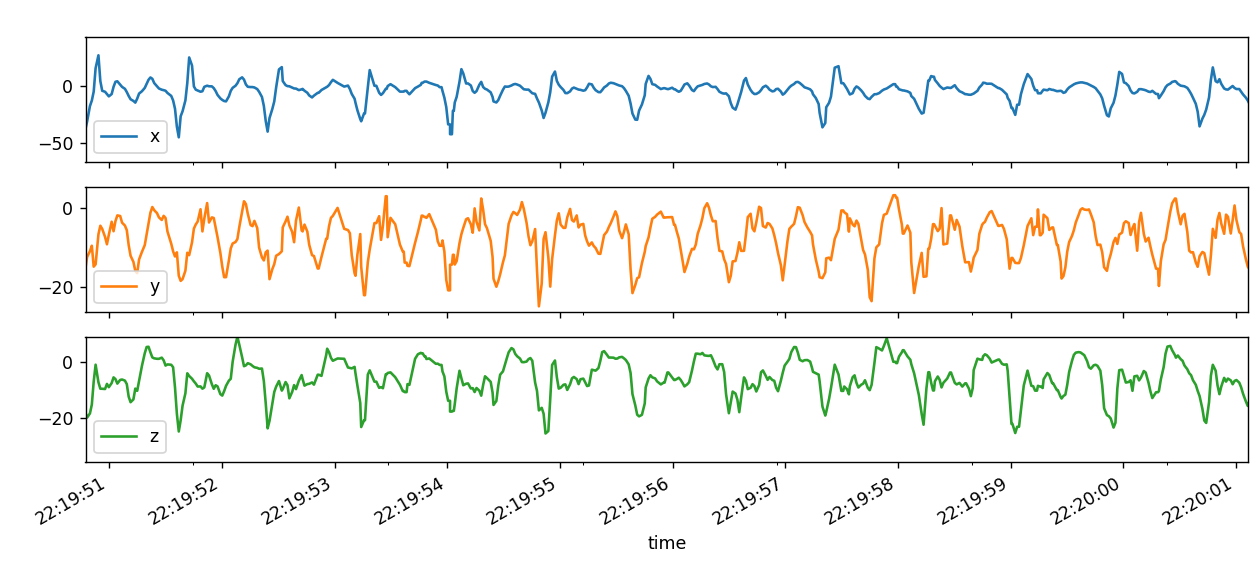
\includegraphics[width=.9\textwidth]{rope_skipping/jump_slow_proefpersoon1.PNG}
\end{figure}

\begin{figure}[!htpd]
\centering
\caption{Proefpersoon 2: springen met tussensprong}\label{fig:jump_slow2}
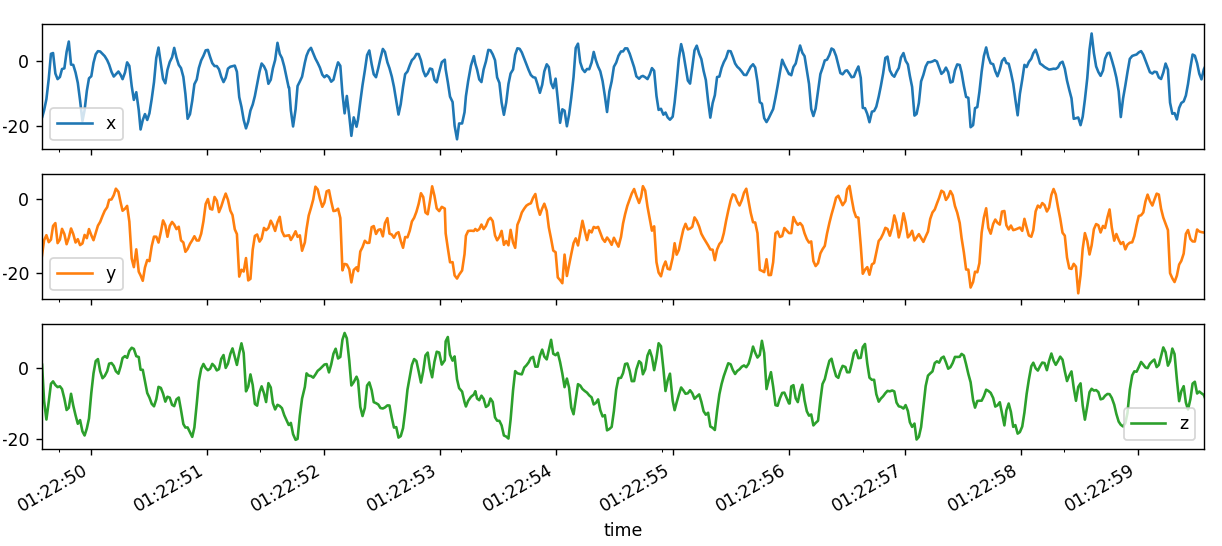
\includegraphics[width=.9\textwidth]{rope_skipping/jump_slow (10 sec).PNG}
\end{figure}

Bij springen met tussensprong zal er met iedere draaiing van het touw twee keer gesprongen worden.
In bovenstaande Figuren is het verloop te zien van de verschillende accelerometer assen tijdens het springen. Er is een duidelijk periodiek verloop merkbaar. Één periode staat gelijk aan één enkele draaiing. 
Door de tussensprong is de periode op alle drie de grafieken schijnbaar opgedeeld in twee stukken. Een tussensprong veroorzaakt namelijk een extra beweging langs alle drie de assen. 
Ook is de versnelling grotendeels negatief wat aangeeft dat er een grotere snelheidsverandering is bij beweging in de richting van de negatieve assen.

\subsubsection{Vergelijking proefpersonen}
Op Figuur \ref{fig:jump_slow1} en \ref{fig:jump_slow2} zijn signalen te zien van twee verschillende proefpersonen die dezelfde sprong uitvoeren. Alhoewel globaal een overeenkomstige vorm terugkeert, zijn er toch duidelijke verschillen merkbaar en dit vooral op de x en z as. Op de z as is te zien dat proefpersoon 1 in de eerste helft van een draaiing een grote versnelling heeft. Bij proefpersoon 2 is dit juist omgekeerd. Op de x as is te zien dat proefpersoon 1 een nagenoeg constante snelheid aanhoudt tijdens een periode. Proefpersoon 2 veroorzaakt op een gegeven moment tijdens een draaiing een kortstondige versnellingspiek. Dit kan te wijten zijn aan het al dan niet uitgesproken zijn van de tussensprong.

\subsection{Springen zonder tussenprong (jump fast)}

\begin{figure}[!htpd]
\centering
\caption{Proefpersoon 1: springen zonder tussensprong}\label{fig:jump_fast1}
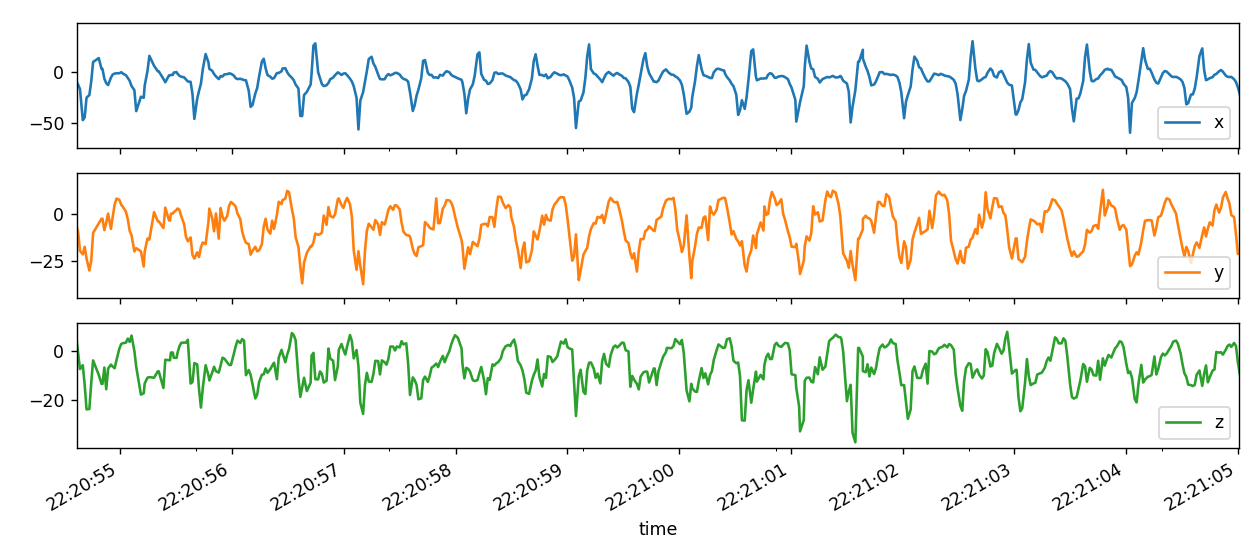
\includegraphics[width=.9\textwidth]{rope_skipping/jump_fast(proefpersoon1).PNG}
\end{figure}

\begin{figure}[!htpd]
\centering
\caption{Proefpersoon 2: springen zonder tussensprong }\label{fig:jump_fast2}
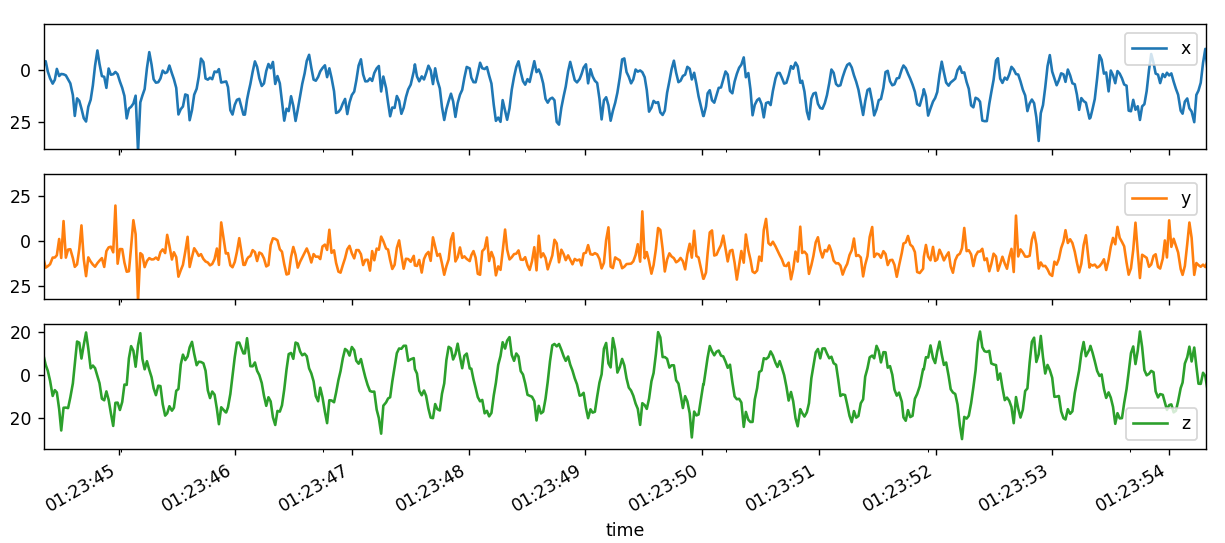
\includegraphics[width=.9\textwidth]{rope_skipping/jum_fast (10 sec).PNG}
\end{figure}

Bij deze beweging vindt er tijdens elke draaiing van het touw één sprong plaats in plaats van twee. Dit resulteert in een kleinere periode en grotere frequentie. 
Het signaal op de x-as is ook weer voor het grootste deel negatief. Dit is niet het geval voor de andere assen.

\subsubsection{Vergelijking proefpersonen}
Figuren \ref{fig:jump_fast1} en \ref{fig:jump_fast2} tonen de accelerometer signalen.
De y-as is een goede indicator voor de grootte van de polsbeweging tijdens een sprong aangezien er minder versnelling zal zijn langs die as bij kleinere draaiingen. Deze as staat namelijk voor het grootste deel van één periode naar boven gericht (zie subsectie \ref{polar}). Proefpersoon 2 maakt bijgevolg kleinere draaiingen in vergelijking met proefpersoon 1.

\subsection{Jump run}

\begin{figure}[!htpd]
\centering
\caption{Proefpersoon 1: jump run}\label{fig:jump_run1}
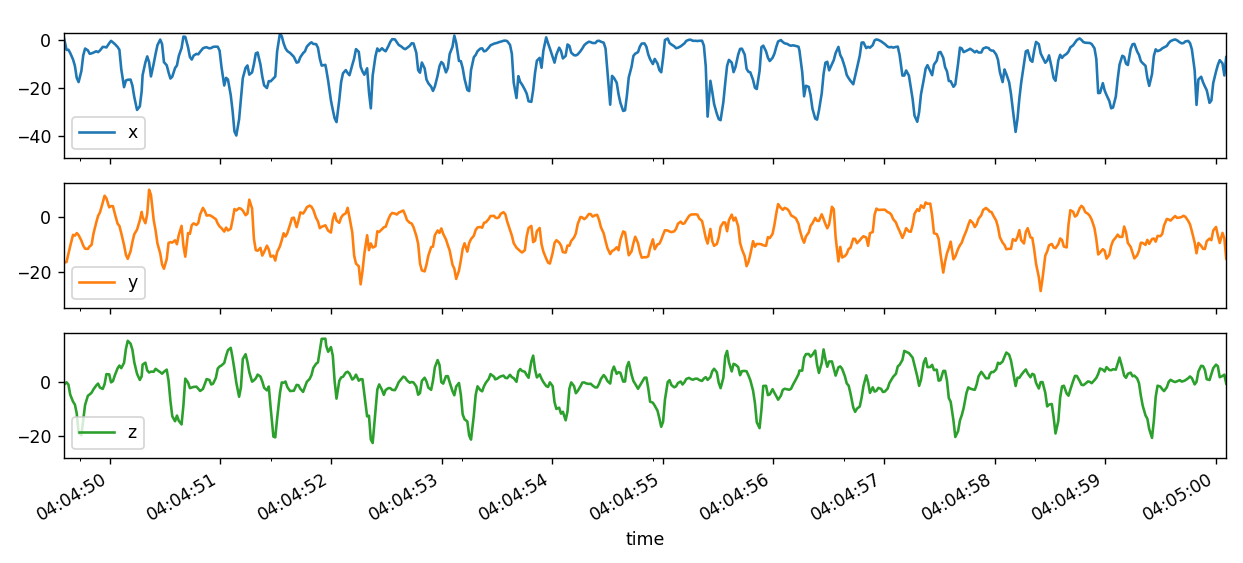
\includegraphics[width=.9\textwidth]{rope_skipping/jump_run_proefpersoon1.PNG}
\end{figure}

\begin{figure}[!htpd]
\centering
\caption{Proefpersoon 2: jump run}\label{fig:jump_run2}
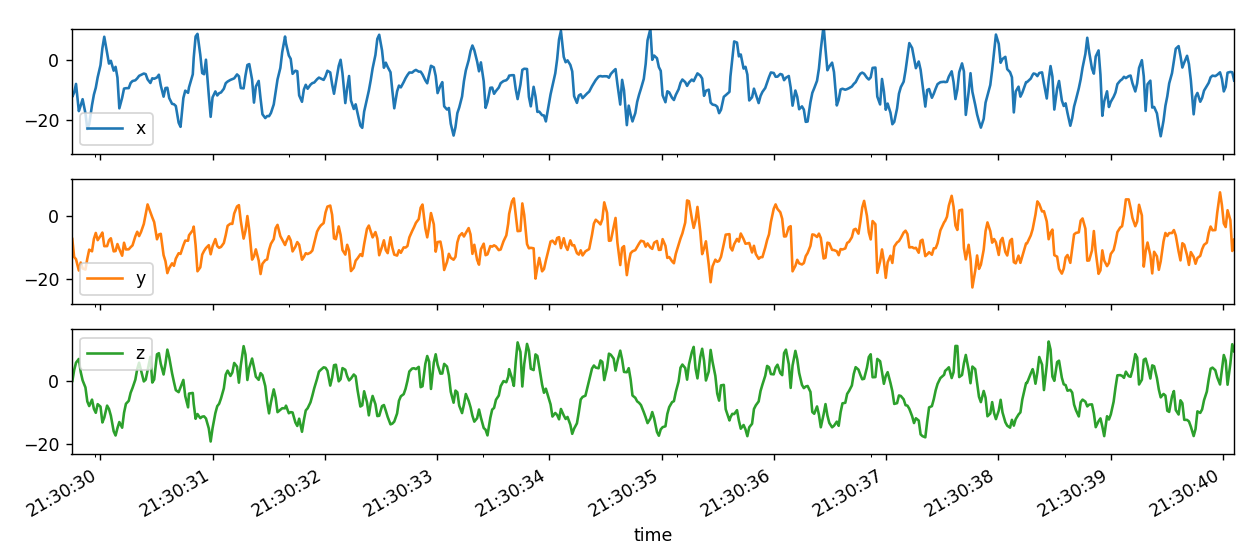
\includegraphics[width=.9\textwidth]{rope_skipping/jump_run_proefpersoon2.PNG}
\end{figure}

Deze beweging is een combinatie van lopen en springen met tussensprong. Er wordt met andere woorden al springend gelopen. Indien deze signalen vergeleken worden met de beweging: springen met tussensprong, dan kan opgemerkt worden dat deze toch wel enige gelijkenissen vertonen. Dit is zeker logisch aangezien een jump run eigenlijk bestaat uit springen met tussensprong aangevuld met verplaatsing. Toch is er een onderscheid en dit is vooral merkbaar op de x-as.

\subsubsection{Vergelijken proefpersonen}
De onderlinge verschillen, te zien op Figuren \ref{fig:jump_run1} en \ref{fig:jump_run2}, zijn gelijkaardig aan deze aangekaart in subsectie \ref{jumpslow}. Aangezien de x-as de meeste verschillen toont, zal deze besproken worden. Proefpersoon 2 vertoont hierbij een grilliger verloop wat aangeeft dat de mate van versnelling vaak verandert langs deze as. 

\subsection{Cross over}

Cross over is een beweging waarbij gesprongen wordt met de armen gekruist. Een illustratie hiervan is te zien op Figuur \ref{fig:crossover}. Tijdens dit onderzoek werd ervoor gekozen om te focussen op cross over met tussensprong. Dit door het tekort aan proefpersonen die in staat zijn de snellere en intensievere versie hiervan uit te voeren.
Op Figuur \ref{fig:cross_over1} is duidelijk te zien dat de amplitude langs de x-as veel kleiner is. De x-as loopt namelijk evenwijdig met de arm en aangezien de armen in een nogal geklemde positie zitten is beweging langs deze as moeilijker (zie subsectie \ref{polar}). Verder is er ook weer een periodiek verloop merkbaar, al is dit wat minder uitgesproken.
X- en y-as ondergaan vooral een versnelling in negatieve richting. De z-as daarentegen ondergaat doorgaans een positieve versnelling.
Aangezien er een tekort aan proefpersonen is die bekwaam zijn om deze beweging uit te voeren, is het niet mogelijk om een onderlinge vergelijking te maken.

\begin{figure}[!htpd]
\centering
\caption{Proefpersoon 1: cross over}\label{fig:cross_over1}
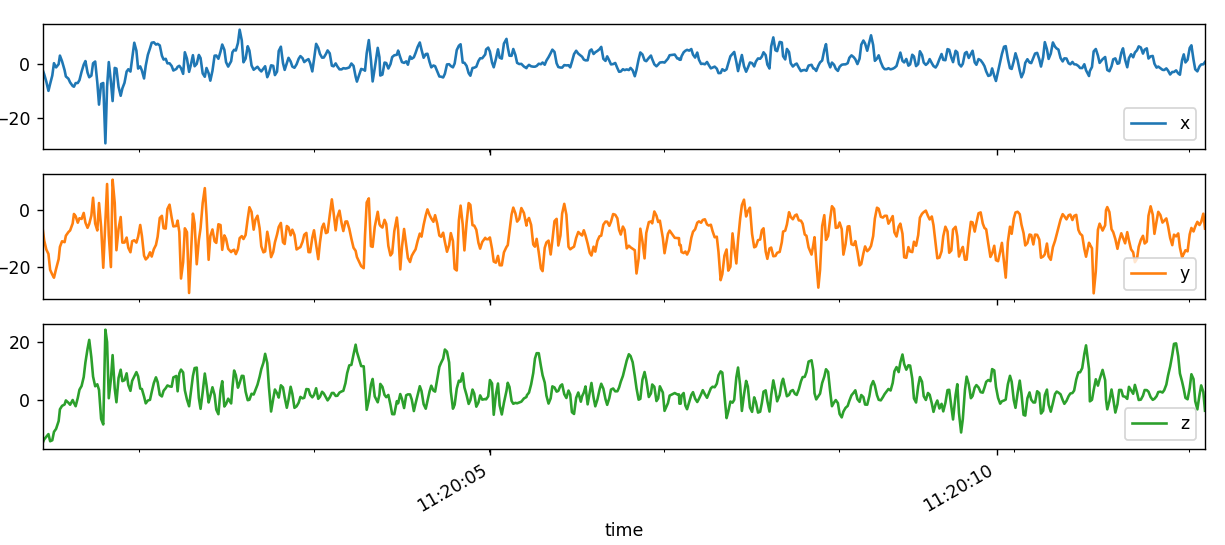
\includegraphics[width=.9\textwidth]{rope_skipping/crossover (10 sec).PNG}
\end{figure}

\subsection{Side swing} \label{subsection:sideswing}

Side swing (zie Figuur \ref{fig:sideswing}) is een beweging waarbij de uitvoerder het touw één maal rechts van hem/haar ronddraait en meteen hierna één maal links. Er kan ook voor gekozen worden om links te beginnen en rechts te eindigen.
Ook in dit signaal is een periodiek verloop merkbaar (zie Figuren \ref{fig:side_swing1} en \ref{fig:side_swing2}). De verandering in snelheid langs de verschillende assen verloopt echter trager. De armen en polsen zijn tijdens deze beweging namelijk compleet vrij zodat op elke as duidelijke veranderingen in richting zichtbaar zijn.
Aan de waarden is te zien dat deze kleiner zijn. Dit komt omdat side swing een rustige beweging is met minder bruuske snelheidsveranderingen. Ook dit verloop is in twee stukken verdeeld op x- en y-as doordat dezelfde beweging langs beide kanten van het lichaam moet uitgevoerd worden. De z-as daarentegen vertoont een ander soort patroon. 

\subsubsection{Vergelijken proefpersonen}
Het verloop van de y- en z-as is zeer gelijkaardig. De x-as daarentegen vertoont enkele verschillen. Proefpersoon 1 toont een duidelijker patroon in vergelijking met proefpersoon 2. Dit tweede signaal bevat namelijk enkele pieken.

\begin{figure}[!htpd]
\centering
\caption{Proefpersoon 1: side swing}\label{fig:side_swing1}
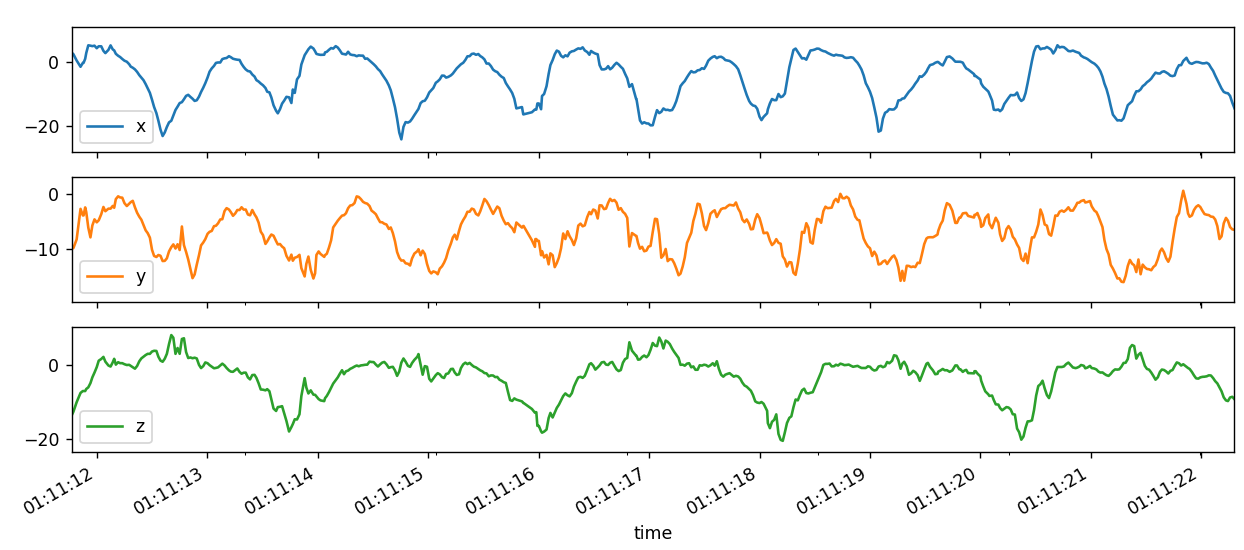
\includegraphics[width=.9\textwidth]{rope_skipping/side_swing_proefpersoon1.PNG}
\end{figure}

\begin{figure}[!htpd]
\centering
\caption{Proefpersoon 2: side swing}\label{fig:side_swing2}
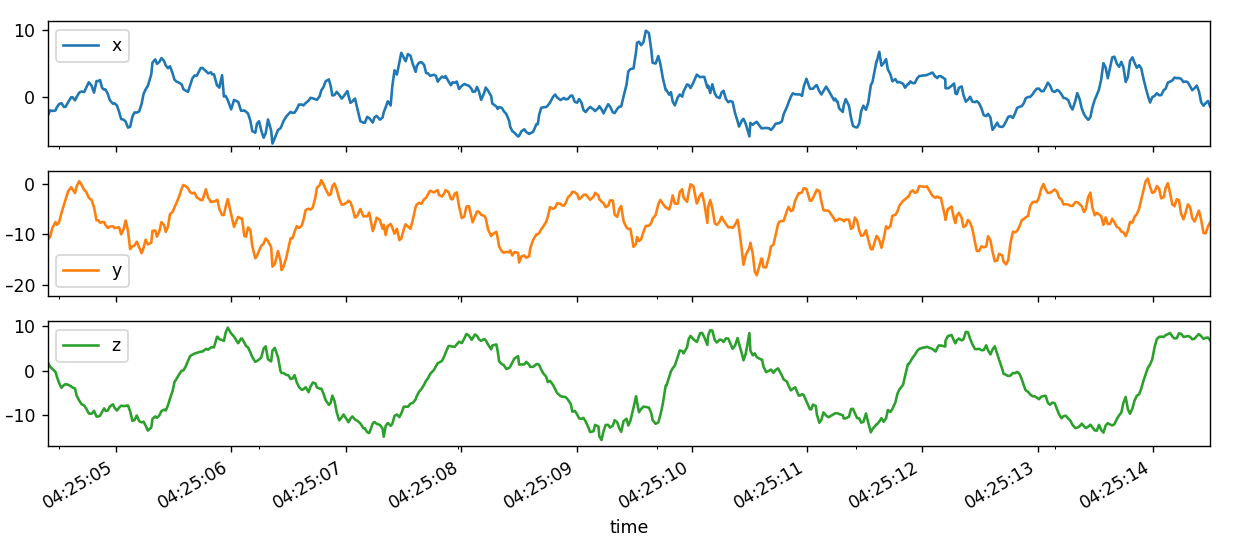
\includegraphics[width=.9\textwidth]{rope_skipping/side-swing (10 sec).PNG}
\end{figure}

\subsection{Forward 180}
Deze beweging zorgt ervoor, zoals de naam zegt, dat de uitvoerder zichzelf 180 graden draait tijdens het springen (zie Figuur \ref{fig:forward180}). Dit wordt verwezenlijkt door met behulp van een side swing tijdens het draaien het touw op de juiste plaats te krijgen. Wanneer men gedraaid is kan achterwaarts verder gesprongen worden.
Het meten van deze beweging was iets moeilijker aangezien dit niet constant achter elkaar kan uitgevoerd worden. Een oplossing bestond erin om na iedere achterwaartse sprong, het touw van richting te veranderen. 
Het periodiek verloop is terug zichtbaar doordat dezelfde beweging telkens opnieuw werd uitgevoerd (zie Figuren \ref{fig:forward_1801} en \ref{fig:forward_1802}).
De ruis die te zien is tussen twee perioden door (vooral langs de y-as) heeft te maken met het feit dat na één beweging, zoals vermeld, van richting moet veranderd worden. De handen moeten bijgevolg terug in positie gebracht worden.
Ook hier is de grafiek weer in twee delen verdeeld. Er zijn tijdens deze beweging eveneens twee sprongen nodig met daartussen een side swing als overgangsbeweging.
De richting van de versnellingsvector is hoofdzakelijk negatief langs de x- en y-as. 

\subsubsection{Vergelijken proefpersonen}
Zoals vermeld bestaat deze beweging uit twee sprongen en een halve side swing. De y-as vertoont een grote gelijkenissen tussen de twee signalen. De x- en z-as vertonen bij proefpersoon 1 een eerder statisch verloop met enkele pieken in tegenstelling tot proefpersoon 2. 

\begin{figure}[!htpd]
\centering
\caption{Proefpersoon 1: forward 180}\label{fig:forward_1801}
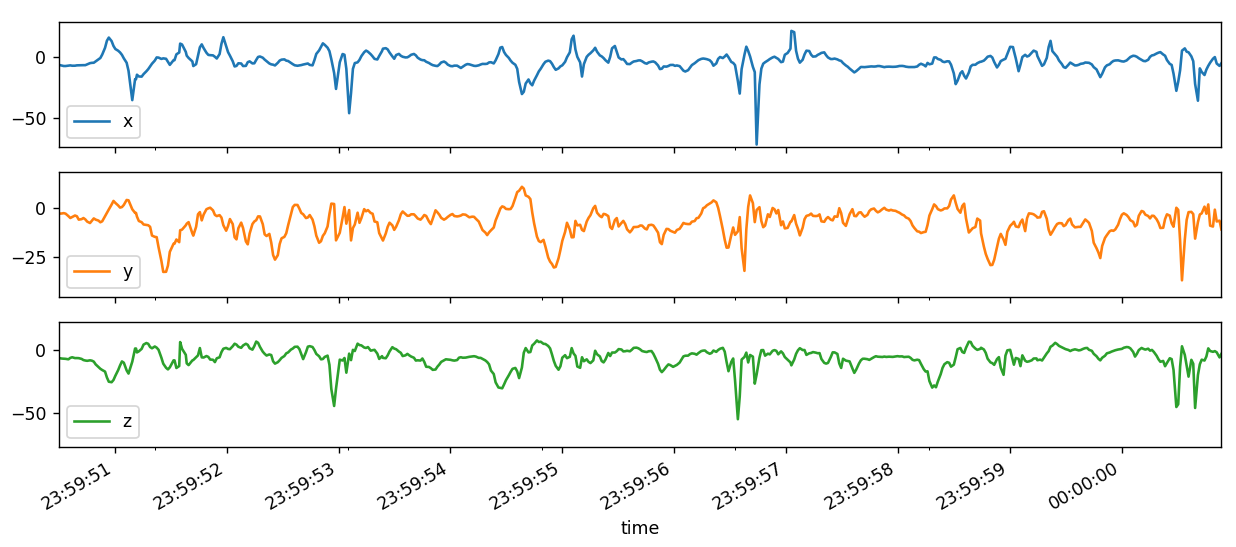
\includegraphics[width=.9\textwidth]{rope_skipping/forward_180_proefpersoon1.PNG}
\end{figure}

\begin{figure}[!htpd]
\centering
\caption{Proefpersoon 2: forward 180}\label{fig:forward_1802}
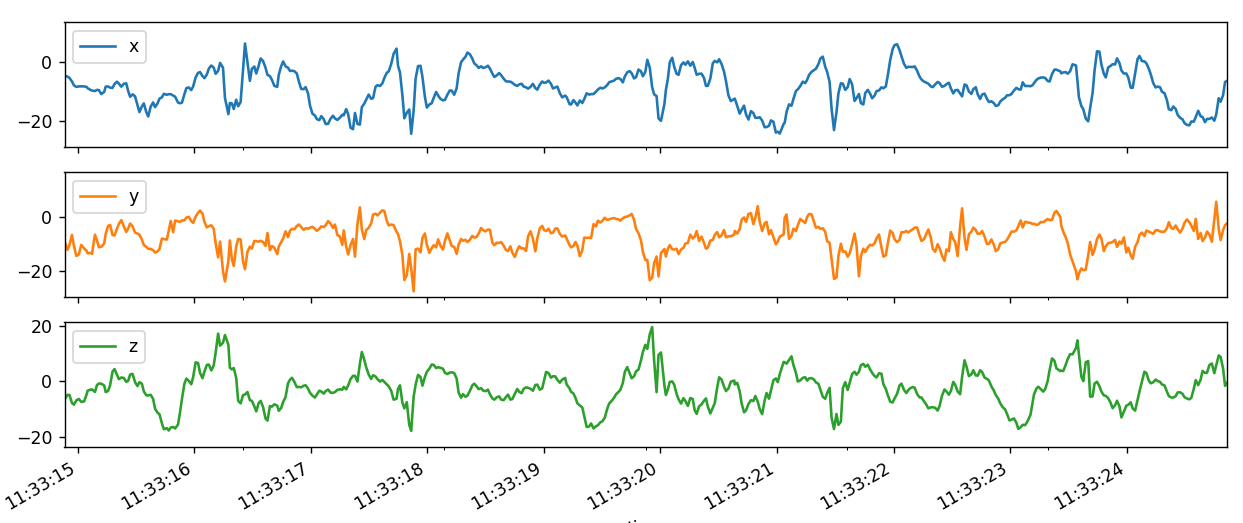
\includegraphics[width=.9\textwidth]{rope_skipping/forward-180 (10 sec).PNG}
\end{figure}

\subsection{Backward 180}
De backward 180 is gelijkaardig aan de forward 180 in zijn uitvoering met als verschil de start-draaiing. Er wordt namelijk gestart vanuit achterwaarts springen. Wanneer het touw zich voor de springer bevindt, draait deze zich 180 graden. Er wordt vervolgens verder voorwaarts gesprongen. Deze beweging bestaat eveneens uit twee sprongen, zonder de aanwezigheid van een halve side swing. Op alle drie de assen is vooral een negatieve versnelling merkbaar. 

\subsubsection{Vergelijken proefpersonen}
Figuren \ref{fig:backward_1801} en \ref{fig:backward_1802} tonen het accelerometer signaal.
De twee signalen lijken in dit geval zeer sterk op elkaar. Enkel komt de iets statischere gedaante van proefpersoon 1 hier weer terug.

\begin{figure}[!htpd]
\centering
\caption{Proefpersoon 1: backward 180}\label{fig:backward_1801}
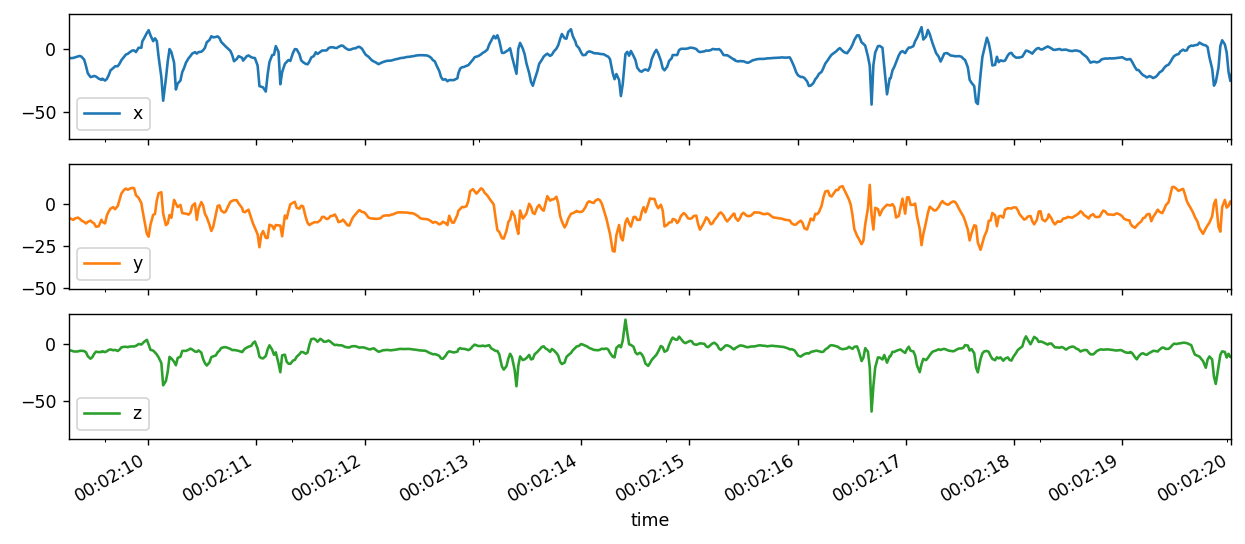
\includegraphics[width=.9\textwidth]{rope_skipping/backward180_proefpersoon1.PNG}
\end{figure}

\begin{figure}[!htpd]
\centering
\caption{Proefpersoon 2: backward 180}\label{fig:backward_1802}
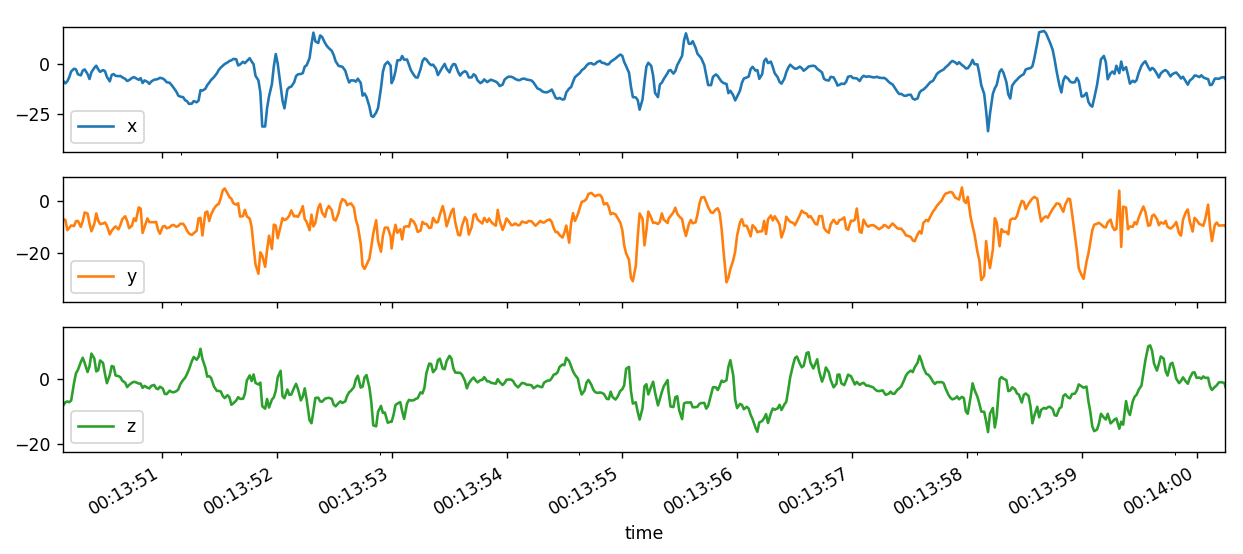
\includegraphics[width=.9\textwidth]{rope_skipping/backward180_proefpersoon2.PNG}
\end{figure}

\begin{figure}[!htpd]
\centering
\begin{floatrow}
  \ffigbox[\FBwidth]{\caption{Cross over \cite{ref82}}\label{fig:crossover}}{%
    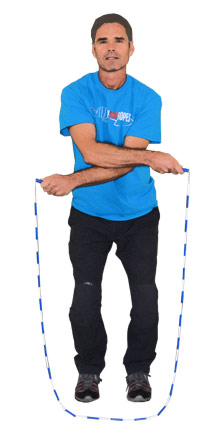
\includegraphics[scale=0.25]{rope_skipping/crossover.jpg} 
  }
  \ffigbox[\FBwidth]{\caption{Side swing \cite{ref82}}\label{fig:sideswing}}{%
    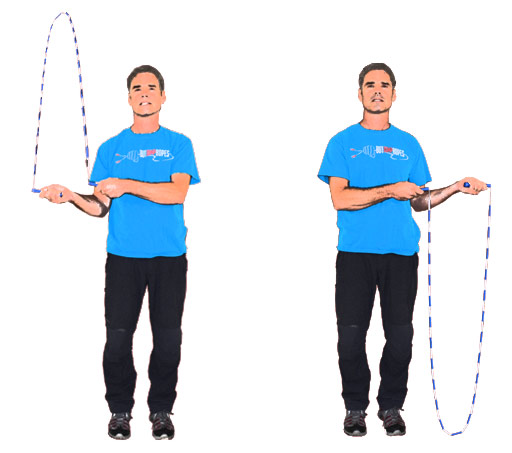
\includegraphics[scale=0.25]{rope_skipping/side-swing.jpg}
  }
  \ffigbox[\FBwidth]{\caption{Forward 180 \cite{ref82}}\label{fig:forward180}}{%
     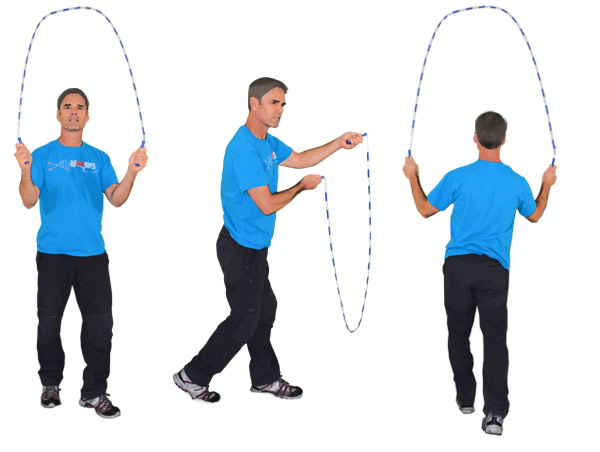
\includegraphics[scale=0.25]{rope_skipping/forward-180.jpg}
  }
\end{floatrow}
\end{figure}

\section{Data collectie} \label{sectie:datacollectie}
Het Polar flow platform laat niet toe om voor een sessie de onbewerkte data te downloaden \cite{ref28}. Hierdoor werd een eigen applicatie ontwikkeld op de smartwatch en smartphone. De smartwatch applicatie zal via sensoren de datapunten opvangen met een sampling frequentie van ongeveer 52 Hz. 

Dit is echter zeer systeem en tijd afhankelijk. Het android systeem en/of andere applicaties kunnen de frequentie ten alle tijde aanpassen. De sampling frequentie kan, afhankelijk van de \textit{lifecycle} waarin de applicatie zit, zelfs verlaagd worden tot 18 Hz \cite{ref68}. Het aantal datapunten per seconde is daarom dus niet stabiel. 
Via een knop op de user interface wordt een sessie gestart, hierna begint de data verzameling. Telkens er een datapunt binnenkomt wordt dit via de wear OS messageClient verzonden naar de smartphone. De datapunten worden op deze manier verzonden omdat ze dan via een applicatie op de android smartphone kunnen opgeslagen worden naar een CSV bestand. Dit is namelijk efficiënter op een smartphone in vergelijking met een smartwatch. Door een andere knop kan de sessie beëindigd worden. Het bestand met data kan dan teruggevonden worden in de externe opslag van de smartphone. Elke applicatie heeft hier in de android/data folder een eigen map. Deze wordt gebruikt voor het opslaan van de bestanden behorend tot de overeenkomstige applicatie.

\section{Preprocessing} \label{section:preprocessing}
Data komende van de smartwatch applicatie bestaat uit vier features: tijd (ns), x-, y- en z-component van de versnelling (m/s²). Dit zonder enige wijziging meegeven aan een machine learning algoritme zal geen goede resultaten geven.
Machines begrijpen onbewerkte data namelijk niet. Data preprocessing biedt hier een oplossing voor. Preprocessing is de aaneenschakeling van stappen die de data zo transformeren dat de features ervan kunnen geïnterpreteerd worden door het algoritme. 
Een dataset is een collectie van data objecten, ook wel records, punten of vectoren genoemd. Data objecten worden beschreven met een aantal features die de basis karakteristieken van het object weergeven. Een feature is hierbij een individueel meetbare karakteristiek van het event dat zich voordeed. 
Bij het bepalen van een activiteit uit accelerometer data worden als features de x- , y- en z-component van het signaal gekozen. Dit zijn namelijk de waarden die het signaal eenduidig kunnen beschrijven. 
Er zijn verschillende types van features. Een eerste onderverdeling wordt gemaakt op basis van het al dan niet numeriek zijn van een feature. 
Een categorische feature is discreet en heeft dus slechts een beperkt aantal mogelijke waarden. Een feature die categorisch is kan nominaal of ordinaal zijn. De aanwezigheid van een zekere ordening onderscheid deze van elkaar. 
Een numerieke feature is continue en wordt gerepresenteerd door nummers. Deze waarden kunnen een interval of ratio beschrijven. Bij een ratio is er sprake van een \textit{true zero}, wat niet het geval is voor interval waarden. Ook zijn negatieve getallen niet mogelijk in geval van een ratio feature. 
De x, y en z componenten van accelerometer data zijn bijgevolg numerieke features van het type interval. Dit betekent dat er bij deze data sprake is van ordening en dat verschillen tussen datapunten een betekenis hebben. Het ratio van twee datapunten heeft dan weer geen betekenis door de afwezigheid van een true zero \cite{ref69}.
 
Niet alle stappen van data preprocessing zijn toepasbaar op elk probleem. Dit is namelijk zeer afhankelijk van het soort data waarmee gewerkt wordt. 
In wat volgt worden de stappen die doorgaans ondernomen worden bij preprocessing besproken. Telkens zal vermeld worden of dit toepasbaar is op de preprocessing van accelerometer data.

\subsection{Data Quality Assessment}
Met onbewerkte data van eender welke oorsprong kunnen veel zaken verkeerd lopen met betrekking tot datatype, ontbrekende waarden enzovoort.
Een eerste preprocessing stap is bijgevolg het type van het tijd feature converteren naar een datetime object. Op die manier kan met de effectieve tijdsverschillen gewerkt worden. 
Door de onstabiele samplingfrequentie (zie sectie \ref{sectie:datacollectie}) is het aantal samples per seconde namelijk onzeker. Daarom is het beter om met tijdsverschillen te werken en alle samples in een tijdsinterval te laten horen bij hetzelfde segment. Later zal blijken dat dit niet mogelijk is bij elk machine learning algoritme (zie subsectie \ref{subsectie:cnn}).

Om de data corresponderend met het aan- en uitzetten van de smartwatch tijdens een meting eruit te kunnen filteren, worden standaard de eerste en laatste datapunten in een interval van 3 seconden verwijderd. Deze datapunten horen namelijk bij geen enkele klasse en zal het machine learning model enkel verwarren.

Data komt meestal van verschillende bronnen die al dan niet betrouwbaar zijn. De data zal in dat geval dus ook in verschillende formaten binnenkomen. Tijdens dit onderzoek wordt slechts één sensor gebruikt. Deze complicatie is bijgevolg niet aanwezig. De betrouwbaarheid van de sensor kan echter wel nog in vraag gesteld worden.

Bij observatie van de data waarden zijn namelijk duplicaten merkbaar. Dit is een fout in het datacollectie proces. Dit is echter geen probleem aangezien duplicaten via het Pandas framework makkelijk kunnen gedetecteerd en verwijderd worden.

Duplicaten worden verwijderd om deze data objecten geen voordeel of bias te geven bij machine learning algoritmen. Eveneens zal meer dan één record met dezelfde data een slecht visueel beeld geven bij plotting.

Ontbrekende waarden werden niet geobserveerd, maar hier moet het systeem toch tegen bestand zijn. \textit{Missing values} komen voor door fouten tijdens de data collectie of door een data validatie regel waardoor bepaalde punten niet geldig zijn. Een eerste manier om hiermee om te gaan is volledige rijen met ontbrekende waarden verwijderen. Als veel datapunten incompleet zijn is deze strategie niet aan te raden. Als slechts een klein percentage van de data punten ermee te kampen heeft dan kan ook gekozen worden voor interpolatie methoden. Hierbij zal de waarde geschat worden aan de hand van de andere beschikbare waarden voor die feature. Men kan eveneens kiezen om de ontbrekende waarde in te vullen met het gemiddelde, de mediaan of de modus van de feature. Data verzameling door sensoren in een smartwatch vergt geen menselijke interactie, waardoor de kans op ontbrekende waarden klein is. Rijen waartoe NaN waardes behoren worden daarom verwijderd. Het gemiddelde of de mediaan is niet zo'n goede keuze aangezien dit een vertekend beeld kan geven. De datapunten hebben vaak een groot bereik waardoor een gemiddelde waarde opgeven tijdens bijvoorbeeld een dalende piek een grote daling met vervolgens een stijging zal veroorzaken.

Een laatste mogelijk probleem waarmee data te kampen heeft zijn inconsistente waarden. Om dit te detecteren is het nodig te weten welk datatype een bepaalde feature heeft en of dit hetzelfde is voor alle data objecten. Dit komt vaak voor bij menselijke fouten en is dus hier niet van toepassing. Toch worden enige voorzorgen genomen door ook in dit experiment de x-, y- en z -kolom te geconverteerd naar float objecten \cite{ref69}.

\subsection{Feature aggregation}
De resulterende dataset wordt initieel onderverdeeld in segmenten van 1 seconde elk met 50 procent overlap. Eén volledige sprong zal namelijk gemiddeld iets minder dan 1 seconde duren. Vandaar de keuze voor een segmentgrootte van 1 seconde. In een volgende sectie zal dit verder onderzocht worden. Partiële segmenten waarin onvoldoende datapunten aanwezig zijn, worden genegeerd.
Deze aggregatie wordt gedaan omdat uit één enkel datapunt weinig info kan gehaald worden. Het verloop in de tijd, de context, is namelijk belangrijk. Aggregaties bieden immers een high level view van de data die stabieler is dan één individueel data object. Door het samennemen van grote hoeveelheden data objecten tot één samenvattend data object is er ook een vermindering van geheugen consumptie en processortijd \cite{ref69}. 
De bekomen segmenten moeten als laatste stap gelabeld worden. Het \textit{targetlabel} in geval van bewegingsherkenning is de uitgevoerde beweging. 

\subsection{Feature sampling}
Met sampling kan de dataset gereduceerd worden waarna een beter maar duurder machine learning algoritme kan gebruikt worden. Sampling moet op zo'n manier gedaan worden dat de eigenschappen van de originele dataset behouden worden: de samples zijn representatief. Dit wordt bekomen door de juiste sample grootte en sampling strategie te kiezen. Bij \textit{simple random sampling} wordt een gelijke selectie waarschijnlijkheid van een entiteit verondersteld. Hierbij zijn 2 variaties: zonder vervanging en met vervanging. Simple random sampling zonder vervanging verwijdert een geselecteerd data object uit de dataset. Simple random sampling met vervanging plaatst dit object terug zodat het bij volgende sampling iteraties kans heeft om nog eens gekozen te worden. Bij ongebalanceerde datasets is de simple random sampling techniek geen goede keuze. Dit betekent namelijk dat de zeldzame data objecten evenveel kans hebben om geselecteerd te worden als de andere. De bekomen dataset na sampling zal dus niet meer overeenkomen met de originele. \textit{Stratified sampling} daarentegen houdt rekening met de originele distributie. Deze techniek verdeelt de dataset in groepen en neemt uit elke groep een gelijk aantal objecten ook al verschilt de groepsgrootte \cite{ref69}.

Sampling is niet toepasbaar bij bewegingsherkenning op basis van accelerometer data. Hoe groter de dataset en hoe meer variatie hierin, hoe accurater de output van het machine learning algoritme zal zijn. Elke vorm van dataset reductie is dus niet wenselijk.

\subsection{Feature extraction}
Enkel de x-, y- en z-component van een acceleratie-vector is voor de meeste algoritmen niet genoeg om correcte voorspellingen te kunnen maken. Daarom worden hier, op basis van de datapunten in een segment, een aantal nieuwe features ontwikkeld. Hierbij horen onder andere statistische features zoals het gemiddelde, de mediaan, het minimum en het maximum. Een aantal complexere features worden in wat volgt meer toegelicht.

\subsubsection{Signal Magnitude Vector}
SMV wordt gebruikt om de graad van bewegingsintensiteit te evalueren. Dit kan een onderscheid leveren tussen verschillende bewegingen op vlak van intensiteitsniveau. Met volgende formule wordt dit berekend \cite{ref17}.
\[
\sum{\sqrt{x^2 + y^2 + z^2}}
\]

\subsubsection{Signal Magnitude Area} 
SMA wordt gebruikt om een meetwaarde te bekomen die het niveau van activiteit weergeeft en dus het onderscheid kan maken tussen perioden van activiteit en inactiviteit.
Het is een statistische meetwaarde die de omvang (magnitude) weergeeft van een veranderende feature. Magnitude is namelijk een maat die ordening aangeeft. In dit geval geeft SMA dus een ordening aan tussen de verschillende segmenten. SMA wordt berekend door de genormaliseerde integraal te nemen van het signaal. Praktisch is het moeilijk om een integraal te berekenen in Python. Daarom wordt gekozen voor een benaderende berekening. Per tijdstip wordt de absolute waarde van de x-, y- en z-component opgeteld. De bekomen waarden worden vervolgens verzameld in een accumulator \cite{ref17} \cite{ref78}.
\[\frac{\sum |x| + |y| + |z| }{#datapunten}\]

\subsubsection{Tilt angle}
Tilt angle is de hoek die een vector maakt met de x-as. Dit wordt berekend met volgende formule \cite{ref77}.
\[
cos\alpha = \frac{ab}{|a||b|}
\]

\subsubsection{Fourrier transformatie}
De fourrier transformatie zal het signaal voorstellen in functie van de frequentie in plaats van de tijd. Uit deze representatie kunnen een aantal zinvolle features gehaald worden waaronder \textit{Power Spectral Density}.

\subsubsection{Power Spectral Density}
PSD is een maat voor de kracht-inhoud in functie van de frequentie. Het toont de kracht van de variaties (energie) als functie van de frequentie. Anders gezegd, op welke frequentie zijn variaties krachtig en op welke minder \cite{ref79}\cite{ref80}.

\subsection{Dimensionality reduction}
Vaak hebben datasets een groot aantal features. Een image processing probleem kan bijvoorbeeld duizenden features hebben. Dimensionality reduction probeert het aantal features te verminderen, maar niet door simpelweg een subset te nemen (\textit{feature subset selection}). Hoe hoger het aantal dimensies, hoe complexer de dataset. Datasets kunnen voorgesteld worden in een assenstelsel met het aantal assen gelijk aan het aantal dimensies. Een groot aantal dimensies is echter moeilijk te modellen en te visualiseren. Dimensionality reduction mapt de dataset bijgevolg op een lagere dimensionele ruimte. Dit wordt gedaan door nieuwe features te creëren die een combinatie zijn van de oude features. De techniek die hiervoor gebruikt wordt is \textit{Principle Component Analysis}.
Data analyse algoritmes werken namelijk beter met lagere dimensionaliteit. Irrelevante features en ruis werden hierbij geëlimineerd \cite{ref69}. 
Doordat vele algoritmen niet kunnen omgaan met een te grote dimensionaliteit wordt dimensionality reduction toegepast tijdens dit onderzoek. Voor het aantal dimensies werd een aantal van 6 gekozen.

\subsection{Feature encoding}
Het doel van data preprocessing is om de data te encoderen zodat het naar een staat kan gebracht worden die de machine begrijpt. Er zijn algemene normen en regels die gevolgd worden bij feature encoding. Nominale features kunnen een één op één mapping ondergaan zoals bijvoorbeeld een permutatie. Ordinale features kunnen een rangbehoudende verandering ondergaan. Interval features kunnen getransformeerd worden met een wiskundige formule waarbij hun nulpunt behouden wordt (fahrenheit naar celsius). Ratio features kunnen geschaald worden met wiskundige formules (lengte naar meters of \textit{feet}) \cite{ref69}. Accelerometer data bestaat uit interval features zoals eerder vermeld. Hierop kan dus normalisatie of een andere schaling toegepast worden (zie sectie \ref{section:preprocessing}).

Algoritmes geïmplementeerd in Scikit Learn hebben vaak gestandaardiseerde data nodig, data die lijkt op een standaard normale distributie. In de praktijk wordt de data getransformeerd door het gemiddelde te verwijderen en het dan te schalen door deling van de standaard deviatie.
Dit is nodig omdat een feature met een variantie niet in dezelfde order als een andere feature op die manier kan domineren. De preprocessing module van Scikit Learn bevat een klasse standardScalar die de transformer API implementeert. Deze berekent het gemiddelde en standaard deviatie op een training set om dan dezelfde transformatie te kunnen uitvoeren op de test data \cite{ref60}.
Standardisatie zal per featurekolom de datapunten schalen. In het geval van detectie gebaseerd op accelerometer data is dit niet wenselijk omdat de distributie van een verzameling datapunten die het model als input krijgt, steeds anders zal zijn. Toch is er een zeker schaling vereist.
Bij het herkennen van activiteiten moeten individuele datapunten met elkaar vergeleken worden. Om geen appelen met peren te vergelijken, moeten de datapunten zo getransformeerd worden dat ze een gelijke distributie hebben. Dit kan verwezenlijkt worden door elk datapunt te normaliseren.

De ground truth labels in de vorm van rope skipping bewegingen moeten eveneens geëncodeerd worden. Dit wordt verwezenlijkt aan de hand van de \textit{labelEncoder} module van Scikit Learn.

\subsection{Data balancering}
Omdat het model geen voorkeur mag ontwikkelen voor een bepaalde klasse, moet de data gebalanceerd zijn. Dit wil zeggen dat er van elke klasse evenveel samples moeten aanwezig zijn. Indien de data ongebalanceerd is en hier wordt geen rekening mee gehouden dat zou het model elke klasse kunnen bestempelen met hetzelfde label en toch meer dan 50\% accuraatheid verkrijgen.
In een eerste fase van het onderzoek werd dit verwezenlijkt door elke klasse even groot te maken als de kleinste. Dit betekent dat bruikbare data genegeerd werd. Daarom is ervoor gekozen om, in een tweede fase van het onderzoek, \textit{data augmentation} toe te passen. Hierbij zullen de kleinere klassen aangevuld worden met kopieën van hun datapunten. Hierbij moet echter opgepast worden voor overfitting (zie subsectie \ref{subsectie:train}).

\subsection{Train/validatie/test} \label{subsectie:train}
Machine learning algoritmes moeten eerst getraind, daarna gevalideerd en vervolgens getest worden. Op basis van de training data wordt het model gebouwd. Hierbij moet opgepast worden voor overfitting. Dit is het verschijnsel waarbij het model perfect traint op de training data, maar hierdoor realistische data niet correct kan classificeren. Underfitting is het omgekeerde en doet zich voor wanneer te grote tolerantie gegeven wordt aan misclassificaties. De validatie data wordt gebruikt om de hyperparameters van het model te kiezen en te verbeteren. De test data heeft als functie om het getrainde en gevalideerde model te testen \cite{ref69}.  

In een eerste fase werd gebruik gemaakt van een klassieke train/test split. Hierbij zal de training en testdata echter te hard lijken op eenander waardoor gemakkelijk hoge accuraatheid gehaald wordt. In een tweede fase werden train, test en validatie datasets onafhankelijk van elkaar gevormd.

\section{Soorten data}
Eenzelfde beweging kan op verschillende manieren gemeten worden. Zo kan het onderscheid gemaakt worden tussen de pols waaraan de smartwatch gedragen wordt of tussen de draairichting. 
Bewegingen zoals forward 180, backward 180 en jump run kunnen niet of moeilijk met een achterwaartse draairichting beoefend worden. Bijgevolg gelden de besproken variaties niet voor deze bewegingen.
Deze variaties includeren in de training data zal resulteren in een beter model. Aangezien deze in essentie dezelfde beweging voorstellen. In wat volgt wordt de data verder geanalyseerd gebruik makend van de beweging springen met tussensprong.

\subsection{Pols}

\begin{figure}[!htpd]
\centering
\caption{Andere pols}\label{fig:anderepols}
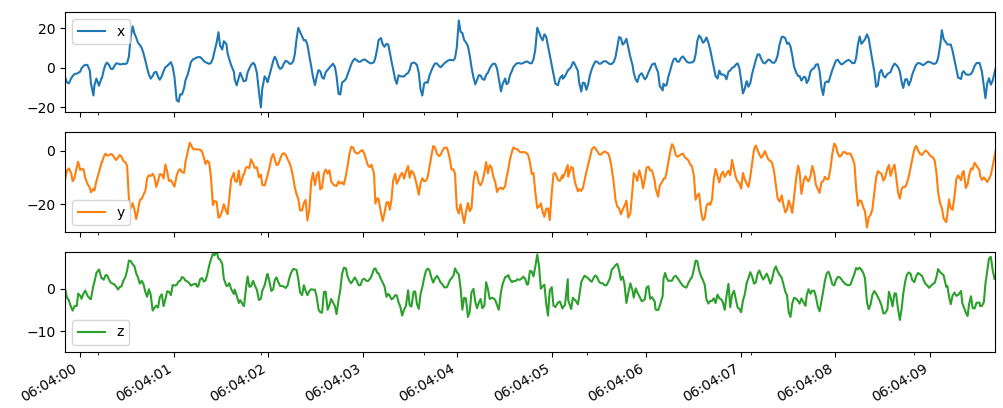
\includegraphics[width=.9\textwidth]{rope_skipping/jump_slow_pols (10 sec).PNG}
\end{figure}

Door de smartwatch aan een andere pols te dragen worden de x- en y-as omgekeerd. Ook zullen ze onder een iets andere hoek komen te staan. De z-component zal alleen onder een andere hoek komen te staan en niet omkeren. Dit resulteert in andere meetwaarden en dus een ander verloop van het signaal (zie Figuur \ref{fig:anderepols}).

\subsection{Draairichting}
\begin{figure}[!htpd]
\centering
\caption{Andere draairichting}\label{fig:anderedraai}
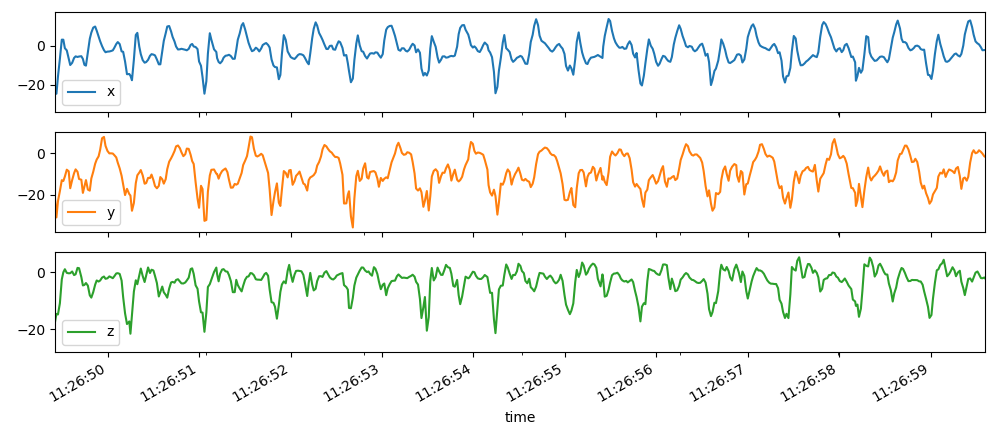
\includegraphics[width=.9\textwidth]{rope_skipping/jump_slow_turn (10 sec).PNG} 
\end{figure}

Een andere draairichting zal de versnellingsvector zelf omkeren terwijl de assen gelijk blijven. Ook hier is er sprake van een gewijzigd verloop van het signaal (zie Figuur \ref{fig:anderedraai}).

\section{Selectie machine learning algoritme}
Machine learning is een modeling techniek gebaseerd op data. Het systeem heeft als input een training set waaruit het model afgeleid wordt. Diversiteit van de training dataset is belangrijk. Een training dataset bestaande uit enkel geschreven nota's van één persoon zal de cijfers/letters van een ander handschrift bijvoorbeeld niet herkennen. Ook is veralgemening van belang. Dit is het proces waarmee de performantie van een model constant gemaakt wordt onafhankelijk van de training of field dataset. Het model zal bijgevolg ook input herkennen die niet volledig overeenkomt met de data waarop getraind werd. 
Er zijn verschillende types machine learning: supervised learning, unsupervised learning en reinforcement learning. Het herkennen van rope skipping bewegingen valt onder supervised learning. Deze techniek zal vanuit een leerverzameling getraind worden om data te herkennen.

Het is belangrijk om het bekomen model correct te evalueren. Zo is geweten of nog meer data of verdere tuning nodig is. Er wordt een score gegeven aan het model waarvoor verschillende metrieken bestaan.
\textit{Accuracy} is het ratio van correct geclassificeerde datapunten en het totaal aantal datapunten. 
\textit{Recall} is het ratio van het totaal aantal correct geclassificeerde positieve samples en het totaal aantal positieve samples. Een positief geclassificeerd datapunt (\textit{true positive}) is een datapunt dat wordt bestempeld met het juiste label. 
\textit{Precision} is het ratio van het aantal correct geclassificeerde positieve samples en het totaal aantal voorspelde positieve samples.
De F1 score is een samensmelting van de recall en precision scores.

Vergelijken van machine learning algoritmes wordt gedaan met confusion matrices. Deze matrices geven een beeld van het aantal \textit{true positives/negatives} en \textit{false positives/negatives}. 

Voor de implementatie van de algoritmes werd grotendeels Scikit Learn gebruikt. Enkel het \textit{convolutional neural network} is afkomstig uit Tensorflow \citep{ref3} \cite{ref29} \cite{ref30}.

In een eerste fase werd het meest optimale model gezocht. Via train test split werd in deze fase een training en test dataset bekomen. Alle modellen naast CNN vereisen meer input dan enkel accelerometer data. Hierdoor werd een groot aantal dimensies bekomen. Deze werden via dimensionality reduction gereduceerd naar 6. In wat volgt wordt de werking van de algoritmen en de resultaten ervan kort besproken. Er werd telkens gebruik gemaakt van \textit{gridSearch} om de meest optimale hyperparameters te bepalen. Het gridSearch algoritme zal namelijk elke combinatie van hyperparameters uitvoeren en degene met de beste accuraatheid teruggeven. Hier werd een window van 1 seconde gebruikt met telkens 50\% overlap.

\subsection{Support Vector Classification}
SVM zorgt voor het maken van een \textit{decision boundary} tussen de verschillende klassen.
In het geval van lineaire scheiding moet ervoor gezorgd worden dat de afstand tussen de boundary en het dichtstbijzijnde datapunt zo groot mogelijk is. Deze decision boundary is een \textit{hyperplane} in een n-dimensionale ruimte waarbij n het aantal features zijn die een datapunt beschrijven. Het hyperplane heeft telkens een dimensie van n-1. Er bestaan veel zulke hyperplanes maar hiervan moet degene gekozen worden met maximale marge.
Bij non-lineaire gevallen wordt gebruik gemaakt van twee concepten: \textit{soft margin} en \textit{kernel tricks}. 
Soft margin wil zeggen dat er een hyperplane gekozen wordt met een aantal verkeerd geclassificeerde datapunten. Hierbij worden twee soorten misclassificaties getolereerd. Een datapunt bevindt zich aan de verkeerde kant van het hyperplane maar wel nog binnen de marge of het datapunt bevindt zich aan de verkeerde kant van het hyperplane en niet binnen de marge. SVM zal dus de balans moeten vinden tussen maximale marge en minimaal misgeclassificeerde datapunten. De hoeveelheid tolerantie die gekozen wordt is een belangrijke hyperparameter. Deze wordt voorgesteld door C in Scikit Learn. Hoe groter C, hoe meer \textit{penalty} het model krijgt bij misclassificatie. De marge zal bij grote C kleiner zijn en er zullen minder \textit{support vectors} zijn. Bij \textit{noisy} data is het dus beter om C niet al te groot te nemen.
Een belangrijk concept hierbij zijn de support vectors. Dit zijn datapunten dichtst bij het hyperplane. De afstand tussen deze vectors moet bijgevolg maximaal gemaakt worden.
De kernel wordt gebruikt om datapunten te herschalen naar een grotere dimensionale ruimte waarin het mogelijk is om de punten met een hyperplane te scheiden. Zo wordt een non-lineaire decision boundary gevonden.
De loss functie, ook wel cost functie genoemd, zal aan elke classificatie een kost toewijzen. 
Door de afgeleide te nemen van deze functie kan gevonden worden in welke richting de gewichten moeten aangepast worden. De gewichten zijn de coördinaten van een vector die loodrecht op het hyperplane staat.
Een regularisatie term kan toegevoegd worden aan de loss functie, deze zal de mate waarin loss wordt toegewezen aan verkeerd geclassificeerde datapunten aanpassen. Op die manier kan overfitting voorkomen worden.

SVC implementeert het \textit{one-against-one} algoritme voor \textit{multiclass classification}. \textit{Classifiers} worden aangemaakt die elk data van 2 klassen trainen. Er zijn dus  n\_class * (n\_class-1)/2 classifiers nodig \cite{ref31}.

De resultaten na toepassing van dit algoritme op de dataset zijn te zien in Figuur \ref{fig:SVC} en Tabel \ref{tab:svc_precision_recall}. Bepaalde klassen worden zeer slecht herkend, andere matig.

\begin{figure}[!htpd]
\centering
\caption{Confusion matrix van SVC}\label{fig:SVC}
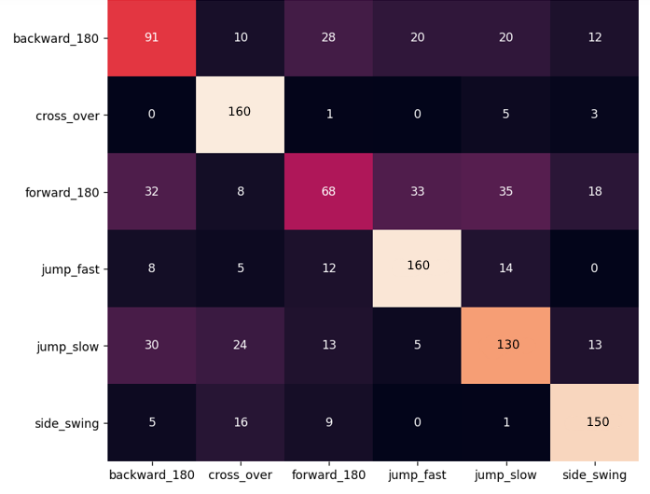
\includegraphics[width=.9\textwidth]{rope_skipping/confusion_matrix_SVC.PNG} 
\end{figure}

\begin{table}[!htpd]
  \centering
  \caption{Precision en recall van SVC}
  \label{tab:svc_precision_recall}
\begin{tabular}{lccc}
 \hline \\
\textbf{}             & \textbf{Precision} & \textbf{Recall} & \textbf{F1} &  \\
\hline \\
\textbf{Forward 180}  & 0.52               & 0.35            & 0.42 & \\
\textbf{Backward 180} & 0.55               & 0.50            & 0.52 & \\
\textbf{Jump slow}    & 0.63               & 0.60            & 0.61 & \\
\textbf{Jump fast}    & 0.74               & 0.80            & 0.77 & \\
\textbf{Cross over}   & 0.72               & 0.95            & 0.82 & \\
\textbf{Side swing}   & 0.77               & 0.83            & 0.80 \\ \\
\hline \\
\end{tabular}
\end{table}

\subsection{Linear Support Vector Classification}

Dit algoritme is vergelijkbaar met SVC indien voor de parameter kernel linear gekozen wordt. Het heeft echter meer flexibiliteit bij het kiezen van penalties en loss functies en zou beter moeten schalen naar grote aantallen samples. 
Support Vector Classifiation doet zijn classificatie, net zoals SVC, door een hyperplane te creëren die de data scheidt in klassen. Hierbij moet de afstand met de support vectors (dit zijn datapunten dichtst bij het hyperplane) maximaal gemaakt worden.
De kernel wordt gebruikt om datapunten te herschalen naar een grotere dimensionale ruimte waarin het mogelijk is om de punten met een hyperplane te scheiden. Zo wordt een non-lineaire descision boundary gevonden. LinearSVC gebruikt een lineaire kernel en vindt dus enkel lineaire decision boundaries.

LinearSVC implementeert de \textit{one-vs-the-rest multiclass} strategie, wat trainen van n\_class modellen betekent. Met optie multi\_class wordt een andere multiclass strategie geselecteerd. Het is echter aangewezen om one-vs-rest te gebruiken aangezien dit algoritme veel sneller is \cite{ref32} \cite{ref33} \cite{ref34}.

De resultaten bekomen na toepassing van linearSVC zijn te zien op Figuur \ref{fig:linearSVC} en Tabel \ref{tab:linearsvc_precision_recall}. De slechtere performantie van dit algoritme was te verwachten aangezien het onderzochte classificatie probleem hoogstwaarschijnlijk niet lineair scheidbaar is.

\begin{figure}[!htpd]
\centering
\caption{Confusion matrix van linearSVC}\label{fig:linearSVC}
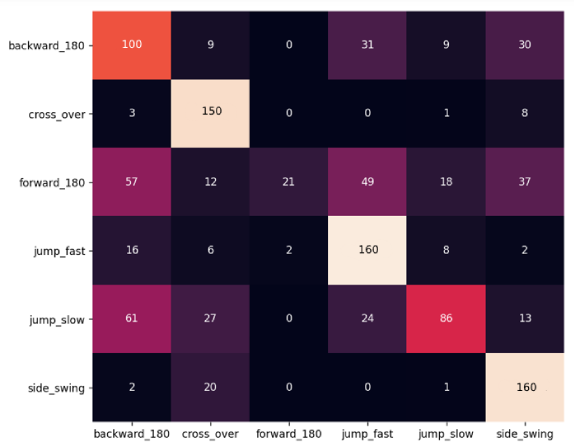
\includegraphics[width=.9\textwidth]{rope_skipping/confusion_matrix_LinearSVC.PNG}  
\end{figure}

\begin{table}[!htpd]
  \centering
  \caption{Precision en recall van linearSVC}
  \label{tab:linearsvc_precision_recall}
\begin{tabular}{lccc}
 \hline \\
\textbf{}             & \textbf{Precision} & \textbf{Recall} & \textbf{F1} &  \\
\hline \\
\textbf{Forward 180}  & 0.91               & 0.11            & 0.20 & \\
\textbf{Backward 180} & 0.42               & 0.56            & 0.48 & \\
\textbf{Jump slow}    & 0.70               & 0.41            & 0.52 & \\
\textbf{Jump fast}    & 0.61               & 0.82            & 0.70 & \\
\textbf{Cross over}   & 0.67               & 0.93            & 0.78 & \\
\textbf{Side swing}   & 0.64               & 0.87            & 0.74 \\ \\
\hline \\
\end{tabular}
\end{table}

\subsection{Random Forest Classifier}
Beslissingsbomen zijn de bouwstenen van het Random Forest model, deze bomen zullen vertakkingen opbouwen aan de hand van features. Er zijn evenveel takken als er mogelijkheden zijn voor waarden van die feature. Random Forest bestaat uit verschillende beslissingsbomen die samenwerken. Elke beslissingsboom in het forest zal een predictie doen. De klasse die het meest voorkomt bij deze predicties wordt de definitieve voorspelling van het model. Er mag geen of geen grote correlatie zijn tussen de verschillende beslissingsbomen. Is dit wel zo dan wordt de kracht van het forest teniet gedaan aangezien het zich nu zal gedragen als één geheel. De verschillende bomen vangen namelijk hun individuele fouten op. Beslissingsbomen zijn zeer gevoelig voor de data waarop ze getraind hebben. Een kleine wijziging hieraan resulteert al in zeer verschillende bomen. Elke boom zal random sampelen met vervanging, hierdoor is de training data van elke boom anders. \textit{Feature randomness} doet zich voor door een proces genaamd \textit{bagging}. Elke boom neemt, bij splitsing van een knoop, de feature die voor het meeste onderscheid zorgt. Dit zal dus ook sterk verschillen tussen bomen.
De belangrijkste hyperparameters zijn de volgende:
Max features geeft de random subset van features weer. Hoe lager dit getal, hoe meer vermindering in variantie en ook hoe meer bias. 
N\_estimators stelt het aantal trees in het bos voor. Naarmate het aantal bomen toeneemt, neemt over het algemeen de fout tot een bepaald punt af. De nauwkeurigheid neemt vanaf dat punt niet meer toe. 
Max\_depth geeft de maximale diepte van iedere boom in het forest aan. Hoe dieper een boom is, hoe meer hoe meer splitsingen er gebeurd zijn en hoe meer informatie over de data aanwezig is.
Min\_samples\_split is het minimum aantal datapunten die nodig zijn om een interne node op te splitsen \cite{ref35}.

De resultaten van dit algoritme zijn te zien op Figuur \ref{fig:random_forest} en Tabel \ref{tab:randomForest}. De performantie is gestegen ten opzichte van eerder bekeken algoritmen. Het zijn echter opnieuw dezelfde klassen die minder goed geclassificeerd worden.

\begin{figure}[!htpd]
\centering
\caption{Confusion matrix van Random Forest}\label{fig:random_forest}
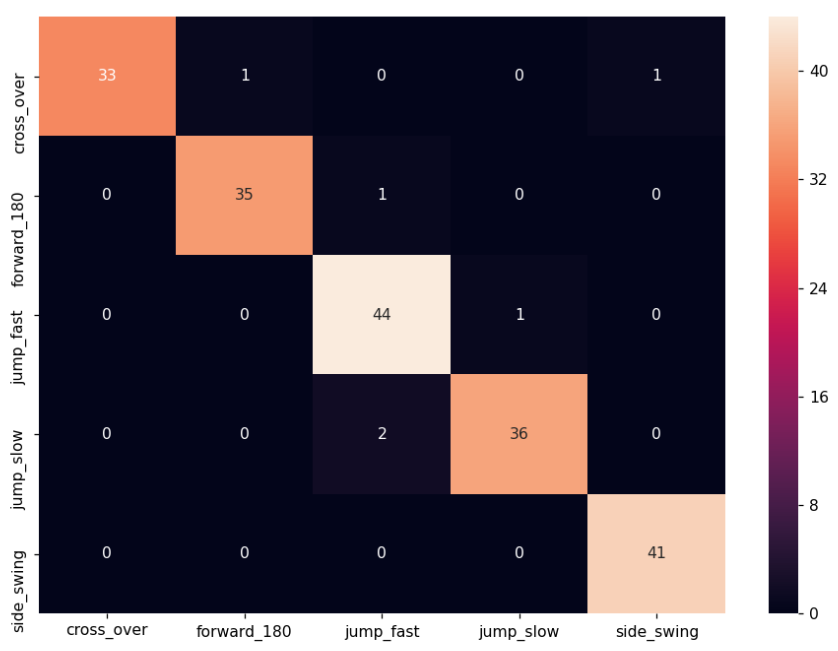
\includegraphics[width=.9\textwidth]{rope_skipping/confusion_matrix_random_forest.PNG}
\end{figure}

\begin{table}[!htpd]
  \centering
  \caption{Precision en recall van Random Forest}
  \label{tab:randomForest}
\begin{tabular}{lccc}
 \hline \\
\textbf{}             & \textbf{Precision} & \textbf{Recall} & \textbf{F1} &  \\
 \hline \\
\textbf{Forward 180}  & 0.63               & 0.53            & 0.58        &  \\
\textbf{Backward 180} & 0.64               & 0.71            & 0.67        &  \\
\textbf{Jump slow}    & 0.68               & 0.68            & 0.68        &  \\
\textbf{Jump fast}    & 0.80               & 0.79            & 0.79        &  \\
\textbf{Cross over}   & 0.82               & 0.90            & 0.86        &  \\
\textbf{Side swing}   & 0.88               & 0.88            & 0.88        & \\ \\
 \hline \\
\end{tabular}
\end{table}

\subsection{AdaBoost}
Adaboost combineert verschillende zwakke classifiers, die slechts lichtjes beter zijn dan \textit{random guessing}, in één sterke classifier. Elke zwakke classifier wordt getraind op een subset van de totale trainingsdata. Deze subsets mogen hierbij overlappen. Elk datapunt krijgt een gewicht toegewezen. Samples met een hoger gewicht hebben meer kans om gekozen te worden. Na training zal Adaboost het gewicht van misgeclassificeerde samples verhogen. Op die manier kan meer aandacht hieraan besteed worden tijdens de volgende iteratie. Classifiers met grotere accuraatheid krijgen meer gewicht. Door de resultaten en gewichten van alle classifiers in rekening te brengen, wordt het Adaboost model bekomen. 

Hoe de zwakke learners geïmplementeerd worden in Adaboost is afhankelijk van hyperparameter base\_estimator. Vaak worden echter beslissingsbomen met één vertakkingsgraad (\textit{decision stumps}) gebruikt. Decision stumps splitsen de dataset in twee gebaseerd op één feature aan de hand van een threshold.

De implementatie in Scikit Learn kan geoptimaliseerd worden met de volgende hyperparameters. Het aantal zwakke learners kan aangegeven worden met de n\_estimators parameter. Hoe meer er van deze aanwezig zijn, hoe complexer de decision boundary is.
De learning rate zwakt de contributie van opeenvolgende iteraties af met een vooraf gedefinieerde factor. Op die manier zal de classifier minder snel leren \cite{ref36}.

Figuur \ref{fig:adaboost} en Tabel \ref{tab:adaboost} geven de resultaten van dit experiment weer. Dit algoritme heeft een gelijkaardige performantie als Random Forest.

\begin{figure}[!htpd]
\centering
\caption{Confusion matrix van Adaboost}\label{fig:adaboost}
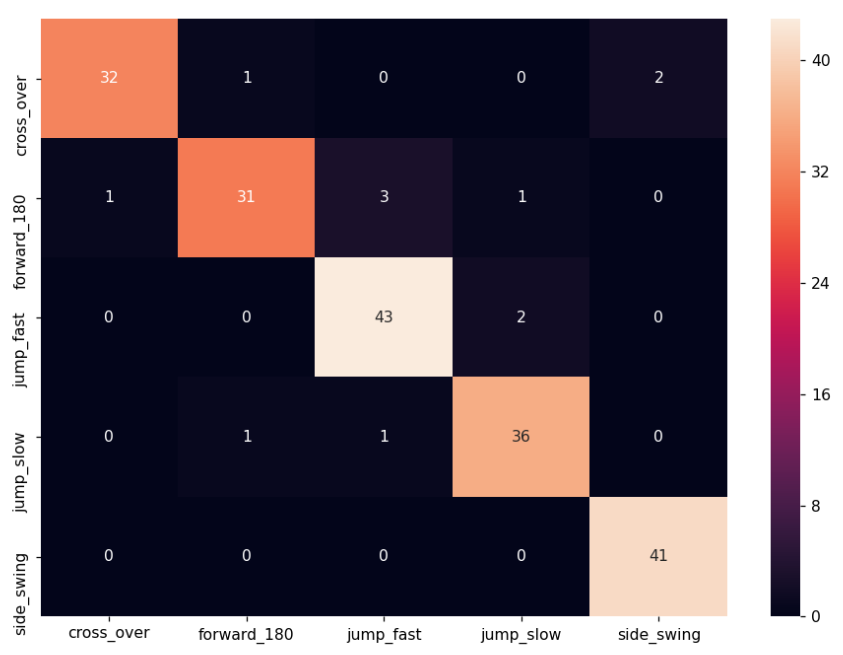
\includegraphics[width=.9\textwidth]{rope_skipping/confusion_matrix_Adaboost.PNG} 
\end{figure}

\begin{table}[!htpd]
  \centering
  \caption{Precision en recall van Adaboost}
  \label{tab:adaboost}
\begin{tabular}{lccc}
 \hline \\
\textbf{}             & \textbf{Precision} & \textbf{Recall} & \textbf{F1} &  \\
\hline \\
\textbf{Forward 180}  & 0.67               & 0.55            & 0.60        &  \\
\textbf{Backward 180} & 0.64               & 0.68            & 0.66        &  \\
\textbf{Jump slow}    & 0.67               & 0.74            & 0.70        &  \\
\textbf{Jump fast}    & 0.79               & 0.77            & 0.78        &  \\
\textbf{Cross over}   & 0.84               & 0.91            & 0.87        &  \\
\textbf{Side swing}   & 0.93               & 0.88            & 0.90        & \\\\
\hline \\
\end{tabular}
\end{table}

\subsection{Naive Bayes}
Naive Bayes is gebaseerd op de Bayes theorie waarbij verondersteld wordt dat de features niet gecorreleerd zijn. 
Naive Bayes berekent de kans dat een feature een bepaalde waarde heeft, gebaseerd op de waarde van een andere feature. 
De klasse met de grootste \textit{posterior probability} is de uiteindelijke voorspelling voor het datapunt. 
Voor elke klasse wordt bijgevolg de kans P(c|f), waarbij c de klasse voorstelt, berekend en dit met elke mogelijke waarde van feature f. 
Naive Bayes is een simpel algoritme dat grote voordelen heeft. 
Er is weinig training data nodig om zeer snel goede resultaten af te leveren. Doordat Naive Bayes geen correlatie veronderstelt tussen de k features moet er geen rekening gehouden worden met de \(2^k\) mogelijke feature interacties.
Hierdoor is Naive Bayes sneller en even performant met kleine datasets in vergelijking met een complex neuraal netwerk. 
Het algoritme presteert goed met categorische variabelen aangezien voor elke waarde van een feature een berekening moet uitgevoerd worden waardoor dit belastend kan zijn in geval van continue variabelen. 
Een ongeziene categorische variabele zal het model echter niet kunnen voorspellen aangezien deze waarden een probabiliteit heeft van 0. 
Er wordt verondersteld dat de features onafhankelijk van elkaar zijn, wat in de praktijk vaak niet zo is.

Parameter alpha geeft aan hoeveel \textit{smoothing} moet toegepast worden op de berekening van de posterior probability. Dit zorgt ervoor dat deze kan nooit nul kan worden \cite{ref37} \cite{ref38}.

Figuur \ref{fig:naive_bayes} en Tabel \ref{tab:naivebayes} visualiseren de resultaten. Deze resultaten laten aan de wensen over vanwege de gebruikte dataset. De vectoren bestaan namelijk uit continue variabelen. Ook is de veronderstelling dat er geen correlatie aanwezig is tussen de features onderling incorrect.

\begin{figure}[!htpd]
\centering
\caption{Confusion matrix van Naive Bayes}\label{fig:naive_bayes}
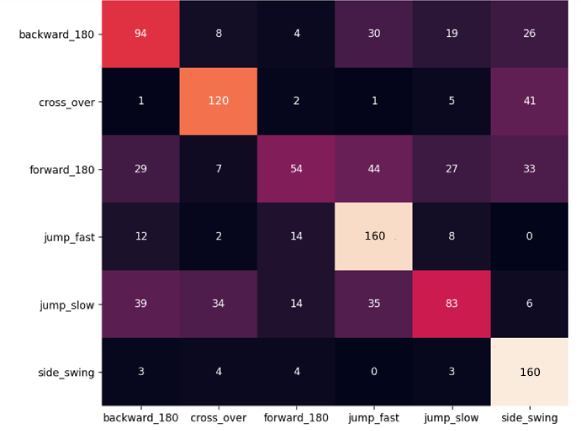
\includegraphics[width=.9\textwidth]{rope_skipping/confusion_matrix_naiveBayes.PNG}  
\end{figure}

\begin{table}[!htpd]
  \centering
  \caption{Precision en recall van Naive Bayes}
  \label{tab:naivebayes}
\begin{tabular}{lccc}
 \hline \\
\textbf{}             & \textbf{Precision} & \textbf{Recall} & \textbf{F1} &  \\
\hline \\
\textbf{Forward 180}  & 0.59               & 0.28            & 0.38        &  \\
\textbf{Backward 180} & 0.53               & 0.52            & 0.52        &  \\
\textbf{Jump slow}    & 0.57               & 0.39            & 0.46        &  \\
\textbf{Jump fast}    & 0.59               & 0.82            & 0.69        &  \\
\textbf{Cross over}   & 0.69               & 0.71            & 0.70        &  \\
\textbf{Side swing}   & 0.60               & 0.92            & 0.73        & \\\\
\hline \\
\end{tabular}
\end{table}

\subsection{K-nearest neighbors}
K-nearest neighbors gaat ervan uit dat gelijkaardige zaken zich in elkaars buurt bevinden. Het algoritme berekent de afstand tussen datapunten gebruikmakend van een bepaalde afstandsmetriek. De euclidische afstand is hierbij de meest voorkomende. 
Het algoritme werkt als volgt: voor elk datapunt wordt de afstand berekend tot alle andere datapunten. Deze afstanden worden vervolgens gesorteerd. 
De meest voorkomende klasse van de k datapunten met de kleinste afstand wordt als voorspelling teruggegeven. 
K is hier de enige en dus ook belangrijkste hyperparameter. 

Dit simpel algoritme heeft zo zijn voordelen. 
Er is slechts één hyperparameter waardoor geen tijd verloren gaat aan het \textit{tunen} van vele parameters. Ook is het bouwen van een complex model niet nodig. 
Bij grote datasets is KNN echter minder performant.

Belangrijke parameters in de Scikit Learn implementatie zijn n\_neighbors, weights, algorithm, leaf\_size en metric.
n\_neighbors stelt k voor. Deze parameter kan een waarde hebben tussen 1 en n-1, waarbij n het aantal datapunten is in de dataset. Een kleine waarde kiezen voor k kan soms onstabiele resultaten geven. Stel dat een datapunt omringd wordt door datapunten van bijna exclusief één bepaalde klasse met slechts een klein aantal behorende tot een tweede verschillende klasse. Liggen de datapunten van deze minder voorkomende klasse toevallig dichterbij dan de rest, dan kan het resultaat met kleine k een vertekend beeld gegeven worden.
Maken we k te groot dan is het mogelijk dat meer misclassificaties ontstaan aangezien ook verder liggende punten in rekening worden gebracht. Een grote k is echter wel in staat om ruis te onderdrukken.
K is best een oneven nummer om geen ex-aequos te vormen.

De weights parameter kan ingesteld worden op uniform of distance. Uniform zal aan alle datapunten evenveel gewicht toekennen.
De configuratie met distance zal de dichtstbijzijnde punten zwaarder laten doorwegen dan punten op een grotere afstand.

De parameter \textit{algorithm} stelt het gebruikte zoekalgoritme in. Doordat telkens alle samples moeten overlopen worden bij classificatie van een nieuw datapunt, is het nuttig om met een efficiënte datastructuur te werken.
Hiervoor zijn enkele opties. Een KD tree is voordelig bij datasets met grote dimensionaliteit maar met een klein aantal datapunten.
Zoeken in deze structuur verloopt echter trager bij grote k.
Een ball tree is nuttig bij zowel grote dimensionaliteit als groot aantal samples. Ook deze structuur presteert slechter bij grote k.

Er kan voor gekozen worden om bij een bepaald aantal datapunten over te schakelen op het brute force algoritme. Dit wordt ingesteld met behulp van de leaf size parameter.

Als laatste kan de gebruikte afstandsmetriek meegegeven worden met behulp van de parameter metric \cite{ref39}.

De resultaten van dit experiment zijn te zien op Figuur \ref{fig:kneighbors} en \ref{tab:kneighbors}. Het is duidelijk dat ook dit algoritme geen match is.

\begin{figure}[!htpd]
\centering
\caption{Confusion matrix van K-nearest neighbors}\label{fig:kneighbors}
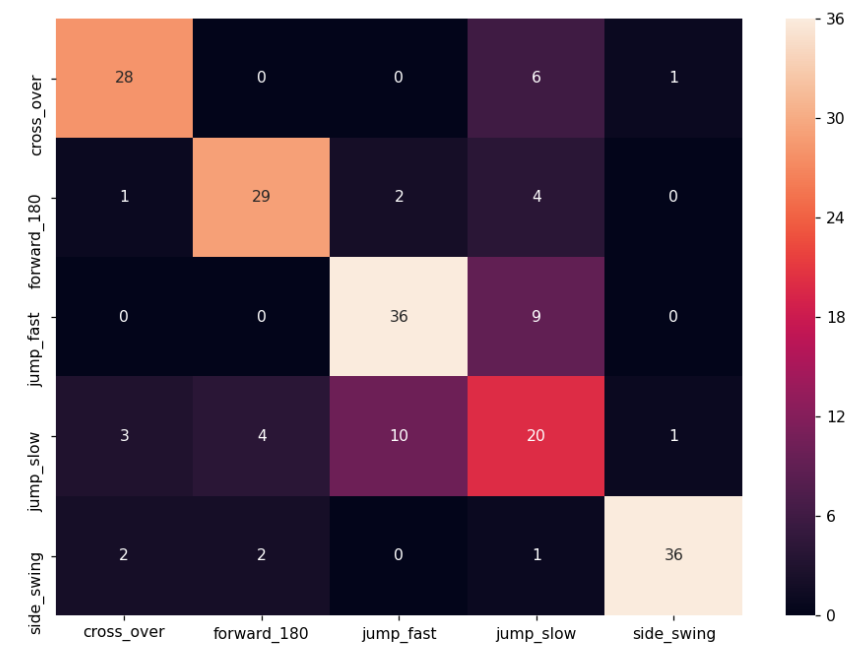
\includegraphics[width=.9\textwidth]{rope_skipping/confusion_matrix_kneighbors.png}   
\end{figure}

\begin{table}[!htpd]
  \centering
  \caption{Precision en recall van K neighbors}
  \label{tab:kneighbors}
\begin{tabular}{lccc}
 \hline \\
\textbf{}             & \textbf{Precision} & \textbf{Recall} & \textbf{F1} &  \\
\hline \\
\textbf{Forward 180}  & 0.38               & 0.30            & 0.34        &  \\
\textbf{Backward 180} & 0.45               & 0.52            & 0.48        &  \\
\textbf{Jump slow}    & 0.51               & 0.34            & 0.41        &  \\
\textbf{Jump fast}    & 0.71               & 0.77            & 0.74        &  \\
\textbf{Cross over}   & 0.71               & 0.88            & 0.79        &  \\
\textbf{Side swing}   & 0.71               & 0.83            & 0.77        & \\\\
\hline \\
\end{tabular}
\end{table}

\subsection{Stochastic Gradient Descent classifier}
De decision boundary wordt, in geval van SGD, voorgesteld door een vector loodrecht op het hyperplane. Door de gewichten van deze vector aan te passen kan de positie van deze boundary veranderd worden. Dit om een optimale classificatie te bekomen. 
Aan de hand van een loss functie wordt berekend wat de totale loss van het model is. Bij misclassificatie wordt aan een datapunt een kost toegekend. De loss functie bepaalt hoe groot deze kost is. Door deze functie dus minimaal te maken kan de meest optimale decision boundary gevonden worden. 
Door de afgeleide te berekenen ten op zichtte van elke feature wordt gekeken in welke richting het hyperplane, in die dimensie, moeten aangepast worden om de minimale kost te bereiken. 
Via een parameter alpha wordt de learning rate meegegeven. Dit geeft aan hoe groot de stappen zijn bij elke update van parameters.
Stochastic gradient descent berekent een benadering voor de gradiënt aan de hand van slechts één datapunt. Dit is efficiënter dan alle datapunten hiervoor te overlopen en pas dan een update door te voeren. Voor grote datasets is dit een zeer goede oplossing. 
De gewichten van het model worden aangepast overeenstemmend met de berekende gradiënt in dat datapunt. 

SGD maakt gebruik van randomness, de training data wordt dus best geshuffeld voor fitting.
Ook wordt de data best geschaald aangezien datapunten met elkaar moeten vergeleken worden.

belangrijke tuning parameters bij dit algoritme zijn alpha, learning rate en max\_iter.
Zoals eerder vermeld geeft alpha weer hoe groot de stappen zijn bij elke update van de model parameters.
Alpha is dus een getal tussen 0 en 1 waarbij een waarde van 1 betekent dat de update totaal niet wordt afgezwakt. 0 betekent dat er geen updates worden doorgevoerd.
Een te grote alpha zorgt ervoor dat het model te snel convergeert naar een niet optimale toestand.
Een te kleine alpha kan ervoor zorgen dat het learning proces vast komt te zitten.

Met de parameter learning rate wordt het \textit{learning rate schedule} bepaald. Het soort schedule geeft weer hoe de learning rate verandert in de tijd.

Het maximum aantal iteraties hangt gedeeltelijk samen met alpha. Bij een kleine learning rate zijn ook meer iteraties nodig \cite{ref40} \cite{ref41} \cite{ref42}.

De resultaten zijn ook hier te zien op Figuur \ref{fig:SGD} en Tabel \ref{tab:SGD}. Deze performantie ligt in lijn met de resultaten bekomen door K-nearest neighbors.

\begin{figure}[!htpd]
\centering
\caption{Confusion matrix van Stochastic Gradient Descent}\label{fig:SGD}
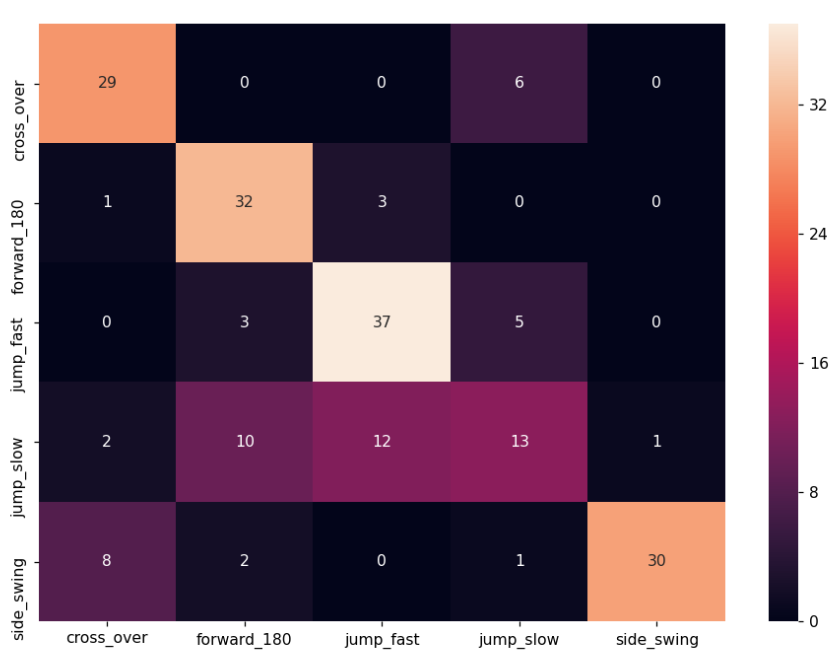
\includegraphics[width=.9\textwidth]{rope_skipping/confusion_matrix_SGD.PNG}  
\end{figure}

\begin{table}[!htpd]
  \centering
  \caption{Precision en recall van SGD}
  \label{tab:SGD}
\begin{tabular}{lccc}
 \hline \\
\textbf{}             & \textbf{Precision} & \textbf{Recall} & \textbf{F1} &  \\
\hline \\
\textbf{Forward 180}  & 0.56               & 0.12            & 0.20        &  \\
\textbf{Backward 180} & 0.46               & 0.48            & 0.47        &  \\
\textbf{Jump slow}    & 0.62               & 0.42            & 0.50        &  \\
\textbf{Jump fast}    & 0.60               & 0.85            & 0.70        &  \\
\textbf{Cross over}   & 0.67               & 0.89            & 0.76        &  \\
\textbf{Side swing}   & 0.59               & 0.86            & 0.70        & \\\\
\hline \\
\end{tabular}
\end{table}

\subsection{Multilayer Perceptron classifier}

MLP is één van de gemakkelijkst te implementeren neurale netwerken.
Een perceptron is de kleinste eenheid van zo'n neuraal netwerk. Dit element zal een aantal inputs met hun corresponderende gewichten vermenigvuldigen en hierbij een bias optellen. Via een activatie functie wordt de output bekomen van de perceptron. Een \textit{multilayer perceptron} bestaat uit minstens drie \textit{nodes} waarvan elk, naast de input node, een non-lineaire activatie functie gebruikt. De nodes tussen de input en output node worden ondergebracht in lagen, \textit{hidden layers} genoemd.

Een loss functie meet de performantie van het netwerk. Een hoge loss betekent dat de voorspelde klasse voor veel datapunten niet correct is. Het is de bedoeling om een set gewichten te vinden die deze loss functie minimaliseert. Het is echter mogelijk dat er meerdere lokale minima voorkomen, verschillende gewicht initialisaties kunnen dus andere resultaten hebben.
De activiatiefunctie beschrijft een non-lineaire relatie tussen input en output. Populaire functies zijn Sigmoid, Relu en Tanh. Het trainen van het model gebeurt in drie fasen: \textit{forward pass, loss calculation} en \textit{backward pass}. Bij de forward pass wordt de input via de lagen doorgegeven waarna uiteindelijk een output wordt berekend. Vervolgens komt een eerste berekening van de loss. Door de partiële afgeleiden te nemen van de loss functie met betrekking tot de verschillende parameters worden de gewichten aangepast (backward pass). In elke laag moet de node die de meeste fouten veroorzaakt heeft beboet worden door hieraan een kleiner gewicht te koppelen.
Muliticlass classificatie wordt mogelijk gemaakt door als laatste laag een Softmax functie te gebruiken.
Een voordeel van deze classifier is de mogelijkheid tot een non-lineaire decision boundary.
Een nadeel is echter dat de loss functie convex is en meer dan één lokaal minimum bevat. Er is eveneens sprake van een grote hoeveelheid hyperparameters. 

Een aantal van de belangrijkste hyperparameters zijn: de gekozen activation functie, alpha en hidden\_layer\_sizes. Alpha stelt de mate van regularisatie in. De hoeveelheid regularisatie bepaalt in welke mate misgeclassificeerde datapunten toegelaten worden.
Met de parameter hidden layer sizes wordt bepaalt van hoeveel hidden layers gebruik gemaakt wordt en hoeveel neuronen in elke laag zitten. Het aantal hidden layers is zeer afhankelijk van de inputdata. Indien deze lineair afscheidbaar is, dan zijn zelfs geen hidden layers nodig \cite{ref43} \cite{ref44} \cite{ref45} \cite{ref46}.

De resultaten na toepassing van dit algoritmen zijn zichtbaar op Figuur \ref{fig:MLP} en Tabel \ref{tab:MLP}. De performantie is iets beter dan K-nearest neighbors, maar kan nog niet tippen aan Random Forest en Adaboost.

\begin{figure}[!htpd]
\centering
\caption{Confusion matrix van Multilayer Perceptron classifier}\label{fig:MLP}
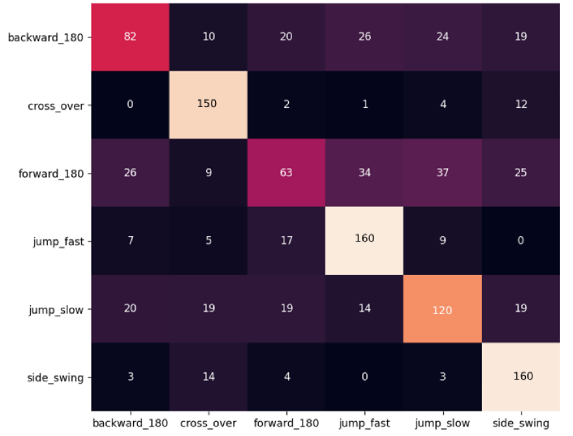
\includegraphics[width=.9\textwidth]{rope_skipping/confusion_matrix_MLP.PNG} 
\end{figure}

\begin{table}[!htpd]
  \centering
  \caption{Precision en recall van MLP}
  \label{tab:MLP}
\begin{tabular}{lccc}
 \hline \\
\textbf{}             & \textbf{Precision} & \textbf{Recall} & \textbf{F1} &  \\
\hline \\
\textbf{Forward 180}  & 0.50               & 0.32            & 0.39        &  \\
\textbf{Backward 180} & 0.59               & 0.45            & 0.51        &  \\
\textbf{Jump slow}    & 0.61               & 0.57            & 0.59        &  \\
\textbf{Jump fast}    & 0.68               & 0.81            & 0.74        &  \\
\textbf{Cross over}   & 0.72               & 0.89            & 0.80        &  \\
\textbf{Side swing}   & 0.68               & 0.87            & 0.76        & \\\\
\hline \\
\end{tabular}
\end{table}

\subsection{CNN} \label{subsectie:cnn}
Dit soort netwerk wordt gekenmerkt door de Convolutional Layer en onderscheidt zich hierdoor van MLP.

Deep learning imiteert de werking van het menselijke brein in de manier van processen van data en maken van patronen voor gebruik in beslissingen. Het is een subset van machine learning en gebruikt hiërarchische levels van artificiële neurale netwerken. Data wordt geprocessed op een niet lineaire manier.
CNN wordt vooral gebruikt bij image processing. In dit geval zijn er veel inputs namelijk het totaal aantal pixels. Voor dit soort problemen kan MLP niet gebruikt worden aangezien voor elke input één perceptron voorzien is wat bij veel data niet echt efficiënt is \citep{ref2}. Het algoritme is echter eveneens toepasbaar op bewegingsherkenning.

Zoals eerder vermeld, is de Convolutional Layer de bouwsteen van een CNN. Convolutie gaat een filter laten glijden over de input array en telkens de convolutie nemen van de overdekte oppervlakte. De convolution layer bestaan uit een aantal afzonderlijke filters.
Het doel hiervan is om features te extraheren. De matrix gevormd door de convolutie uit te voeren met de filter en het dot product te berekenen met de gewichten wordt de activation map of feature map genoemd.

De Pooling Layer is een tweede bouwsteen van CNN. Hiermee wordt de grootte van de representatie gereduceerd aangezien dit resulteert in minder parameters en dus minder rekenwerk. Dit kan aanzien worden als een soort dimensionality reduction. Max pooling, één van de pooling technieken, wordt het meest gebruikt. Hierbij wordt een oppervlak bekeken waaruit enkel de maximum waarde behouden wordt. Door het aantal parameters te reduceren wordt overfitting voorkomen. Dit proces maakt het netwerk eveneens robuust tegen kleine variaties in input data.

Een andere veel gebruikte laag is Relu. Dit is een non-lineaire operatie. De data die het model moet leren zal hoogstwaarschijnlijk non-lineair zijn daarom is het introduceren van non-lineariteit noodzakelijk. Er bestaan ook andere non-lineaire operatie (Tanh en Sigmoid). Relu geeft echter betere resultaten.

Een Fully Connected Layer is een traditionele MLP laag met een Softmax activatie functie in de output layer. Fully connected wil zeggen dat elk neuron uit de vorige laag geconnecteerd is met elke neuron in de laag die erop volgt.
Deze geconnecteerde laag gebruikt de high level features bekomen uit de pooling en convolutie lagen met als doel deze te classificeren. 

In eerste instantie worden de filters en gewichten random geïnitialiseerd. Na de \textit{forward propagation} fase wordt de loss van het model berekend. De gewichten worden geüpdatet door de gradiënt ten opzichte van elke parameter te berekenen. Zo is geweten in welke richting deze moet aangepast worden. In de \textit{backward propagation} fase worden de gewichten effectief ge-update \cite{ref47} \cite{ref48}.

Om overfitting te voorkomen kan gebruik gemaakt worden van een Dropout laag. Deze laag zal bij iedere iteratie een vooraf opgegeven aantal neuronen negeren \cite{ref49}.

Doordat de \textit{input shape} telkens gelijk moet zijn, kan hier niet gewerkt worden met een variërende segmentgrootte. Hierdoor wordt dit gelijkgesteld aan een gemiddelde waarde van 52 samples.

De resultaten van CNN zijn te zien op Figuur \ref{fig:CNN} en Tabel \ref{tab:CNN}. Dit zijn de best bekomen resultaten tot nu toe. Bijgevolg wordt dit algoritme verder geoptimaliseerd.

\begin{figure}[!htpd]
\centering
\caption{Confusion matrix van CNN}\label{fig:CNN}
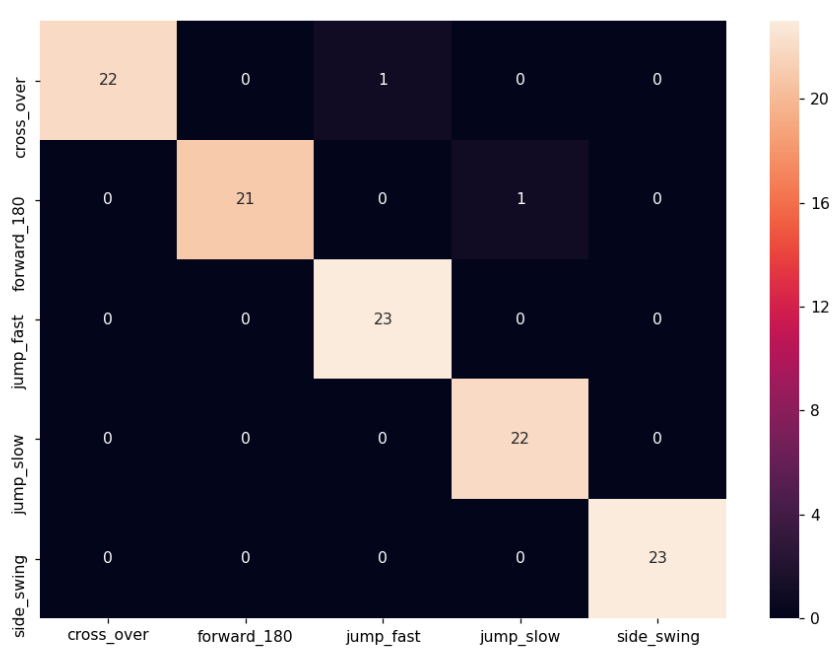
\includegraphics[width=.9\textwidth]{rope_skipping/confusion_matrix_CNN.PNG} 
\end{figure}

\begin{table}[!htpd]
  \centering
  \caption{Precision en recall van CNN}
  \label{tab:CNN}
\begin{tabular}{lccc}
 \hline \\
\textbf{}             & \textbf{Precision} & \textbf{Recall} & \textbf{F1} &  \\
\hline \\
\textbf{Forward 180}  & 0.79               & 0.79            & 0.79        &  \\
\textbf{Backward 180} & 0.86               & 0.86            & 0.86        &  \\
\textbf{Jump slow}    & 0.90               & 0.82            & 0.86        &  \\
\textbf{Jump fast}    & 0.87               & 0.95            & 0.91        &  \\
\textbf{Cross over}   & 0.97               & 1               & 0.98        &  \\
\textbf{Side swing}   & 1                  & 0.96            & 0.98        & \\\\
\hline \\
\end{tabular}
\end{table}

\section{CNN optimalisatie}
Met de klassieke train test split bleek CNN veruit de beste resultaten af te leveren. Dit was in eerste instantie niet zo. Dit kwam echter door een fout in het preprocessen van de data. Voor het maken van segmenten werden de verschillende datapunten geshuffeld. Dit resulteerde in een volledig random model. Wanneer deze fout eruit gehaald werd, werden de resulaten te zien op Figuur \ref{fig:CNN} bekomen. Er werd dus verder gewerkt met dit algoritme. 
Tijdens het trainen van het model werd een callback-functie gebruikt die telkens de beste epoch, deze met de laagste loss, opslaat. Op deze manier wordt steeds het best mogelijke model behouden.
Er werd eveneens besloten om de forward en backward 180 op een andere manier te meten. Oorspronkelijk werd enkel de zuivere beweging gemeten, maar dit is niet realistisch en onnatuurlijk. Tijdens de nieuwe metingen werd een sprong voor de 180 en erna uitgevoerd. Dit is echter ook niet realistisch en zorgde voor meer verwarring in het model. Daarom werd ervoor gekozen om deze beweging niet verder de onderzoeken in het kader van deze thesis.
De redenering achter deze keuze is de volgende. De uiteindelijke gezondheidsapplicatie zal sessies van één bepaalde activiteit aanbevelen. De forward en backward 180 zijn echter bewegingen die moeilijk periodiek kunnen uitgevoerd worden. Ook bleek er grote verwarring tussen backward 180, forward 180 en jump slow onderling. Dit is deels te wijten aan de nieuwe meetwijze dewelke bestaat uit toevoeging van een extra sprong voor en na de backward en forward 180. 
Om het verlies van de forward 180s te compenseren werd gezocht naar een vervangbeweging. De jump run is een goede kandidaat. Uit de vergelijking van de signalen van de jump run, jump slow en jump fast is ook een verschil merkbaar. 

\subsection{validatie dataset}
In een volgend experiment werd een validatie dataset ingevoerd. Deze validatie dataset zal ervoor zorgen dat overfitting van het model voorkomen wordt \cite{ref81}. Tijdens het leerproces zal het netwerk telkens zijn gewichten aanpassen door ook rekening te houden met de validatie data.
Een eerste validatie dataset bestond uit een aantal "scenarios". Tijdens zo'n scenario voert de springer verschillende sprongen door elkaar uit die dan in \textit{postprocessing} geknipt en gelabeld worden.
Het onderscheiden van bepaalde bewegingen in het signaal bleek zeer moeilijk. Om deze reden werd geopteerd voor een validatiedataset bestaande uit periodiek uitgevoerde bewegingen.

\subsection{Window}
Eén van de hyperparameters waaraan kan gesleuteld worden is het window. Tijdens voorgaande experimenten werd standaard gewerkt met een window van één seconde. Dit omdat één enkele sprong steeds een duur heeft van ongeveer één seconde. In Tabel \ref{tab:window} is de accuraatheid ten opzichte van window grootte af te lezen. Deze accuraatheid is een gemiddelde score. Iedere run met een neuraal netwerk levert namelijk verschillende resultaten door de random initialisatie. Aangezien zoals vermeld één sprong een gemiddelde duur van één seconde heeft, is het logisch dat een window van een halve seconde iets minder goede resultaten geeft. Een window groter dan één seconde zal voor problemen zorgen wanneer verschillende bewegingen kort op elkaar volgen. Er zal dan meer dan één beweging aanwezig zijn binnen het window. Om deze reden werd geopteerd voor segmenten van één seconde.

\begin{table}[!htpd]
  \centering
  \caption{Window}
  \label{tab:window}
\begin{tabular}{lccccc}
 \hline \\
\textbf{}         & \textbf{0.5 s} & \textbf{1 s} & \textbf{1.5 s} & \textbf{2 s} & \textbf{3 s} \\
 \hline \\
\textbf{Accuracy} & 0.83           & 0.90         & 0.89           & 0.92         & 0.93  \\\\
 \hline \\
\end{tabular}
\end{table}

\subsection{Overlapping}
Verder werd geëxperimenteerd met al dan niet overlappende segmenten tijdens het trainen. Voorgaande experimenten werkten telkens met 50\% overlap van zowel training en validatie dataset. Een zekere overlapping zal ervoor zorgen dat enerzijds meer trainingsdata ter beschikking is en anderzijds alle karakteristieken van het signaal gemodelleerd worden. Een te grote overlapping zal echter overfitting veroorzaken \cite{ref81}. Dit fenomeen is te zien in Tabel \ref{tab:overlap}. Er werd gekozen om verder te werken met een overlap van 30\%.

\begin{table}[!htpd]
  \centering
  \caption{Overlapping}
  \label{tab:overlap}
\begin{tabular}{lcccc}
 \hline \\
\textbf{}         & \textbf{0\%} & \textbf{30\%} & \textbf{50\%} & \textbf{70\%} \\
\hline \\
\textbf{Accuracy} & 0.88         & 0.93          & 0.90          & 0.93    \\\\
\hline \\
\end{tabular}
\end{table}

\subsection{Splitsen}
Een volgend experiment bestond uit het opsplitsen in meerdere modellen op basis van de variaties in de trainingsdata. Er werden vier modellen getraind, elk gespecialiseerd in één bepaalde soort data. Eén van de model werd getraind op enkel data gemeten aan de rechterpols en in de achterwaartse draairichting, een ander enkel op data gemeten aan de linkerpols en in de achterwaartse draairichting enzovoort. Dit experiment werd inclusief de forward en backward 180 bewegingen uitgevoerd. Deze hebben echter een andere variatie in de vorm van draairichting. Er kan namelijk een draaiing van 180 graden gemaakt worden in twee  richtingen. De accuraatheid steeg hierdoor in de meeste modellen. Er was echter enige verwarring tussen backward en forward 180, wat logisch is aangezien met de nieuwe metingen beide sprongen een jump slow omvatten. 
Met de implementatie van de android applicatie in het achterhoofd werd ervoor gekozen om één model te trainen. In het geval van vier modellen getraind op verschillende data zou de gebruiker telkens moeten opgeven welke variatie men uitvoert (linkerpols-achterwaarts, rechterpols-voorwaarts...). Hierdoor is deze aanpak zeker niet gebruiksvriendelijk.

\subsection{Samenvoegen klassen}
De redenering achter het splitsen van jump slow en jump fast is de volgende. Deze bewegingen vertonen onderling genoeg onderscheid om apart geclassificeerd te worden. Ook steunt de berekening van het aantal draaiingen op dit onderscheid. De gebruikte parameters zijn hierbij verschillend. Bij wijze van experiment werd een samenvoeging van deze klassen uitgevoerd. In Tabel \ref{tab:samenvoegen} is te zien dat dit de classificatie voor het model toch enigszins bemoeilijkt.

\begin{table}[!htpd]
  \centering
  \caption{Samenvoegen jumps}
  \label{tab:samenvoegen}
\begin{tabular}{lccc}
 \hline \\
\textbf{}             & \textbf{Precision} & \textbf{Recall} & \textbf{F1} &  \\
\hline \\
\textbf{Jump run}  & 0.64               & 0.79            & 0.71        &  \\
\textbf{jump}       & 0.97               & 0.87           & 0.92        &  \\
\textbf{Cross over}   & 0.27               & 1               & 0.43        &  \\
\textbf{Side swing}   & 0.79                  & 0.99           & 0.88        & \\\\
\hline \\
\end{tabular}
\end{table}

\subsection{Ensemble learning}
Ensemble learning is een manier om fouten van individuele modellen teniet te doen. Elke nieuwe run van eenzelfde model zal namelijk nooit gelijk zijn met een vorige. Dit door random gewicht initialisaties (zie subsectie \ref{subsectie:cnn}). Vier modellen worden op dezelfde manier getraind met dezelfde input data. Deze modellen zullen samenwerken om tot een oplossing te komen op volgende manier. Wanneer een model een predictie doet, dan wordt aan elk van de klassen een probabiliteit toegekend. Deze probabiliteiten, komende van de vier modellen, worden opgeteld waardoor elk model zijn bijdrage levert tot het uiteindelijke resultaat. De klasse met de hoogste score wordt toegekend aan het segment. Het resultaat hiervan is op Figuur \ref{fig:ensemble} en in Tabel \ref{tab:ensemble} te zien.

\begin{figure}[!htpd]
\centering
\caption{Ensembled model}\label{fig:ensemble}
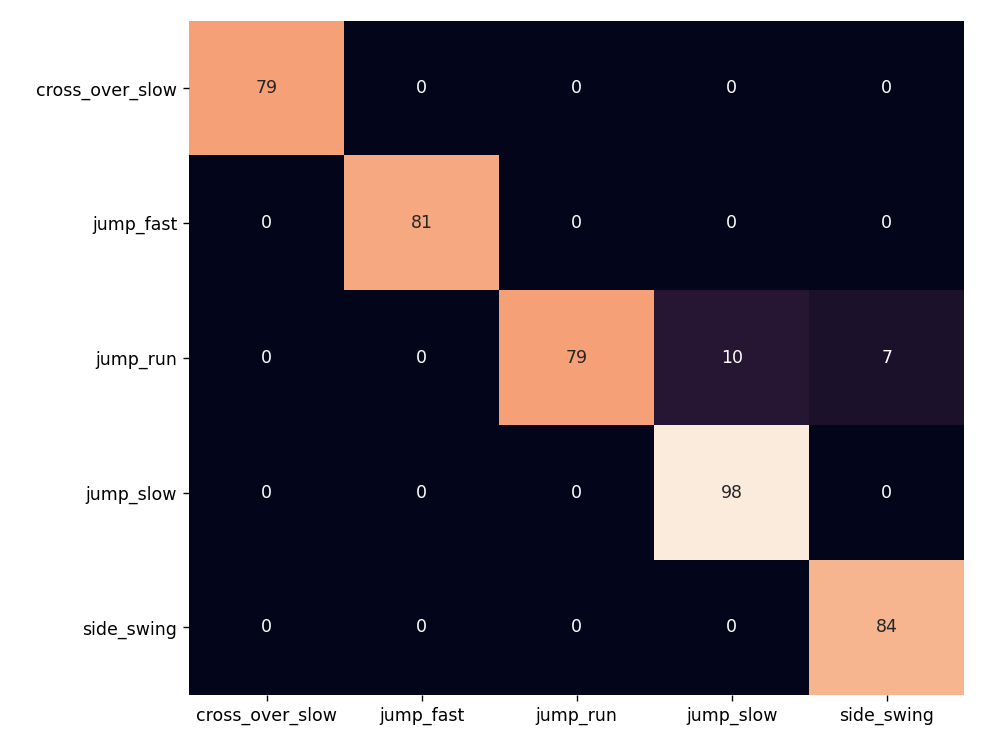
\includegraphics[width=.9\textwidth]{rope_skipping/confusion_matrix_final.PNG} 
\end{figure}

\begin{table}[!htpd]
  \centering
  \caption{Ensembled model performantie}
  \label{tab:ensemble}
\begin{tabular}{lccc}
 \hline \\
\textbf{}             & \textbf{Precision}  & \textbf{Recall}   & \textbf{F1} &  \\
\hline \\
\textbf{Jump run}     & 1                   & 0.82              & 0.90       &  \\
\textbf{Jump slow}    & 0.91                & 1                 & 0.95       &  \\
\textbf{Jump fast}    & 1                   & 1                 & 1       &  \\
\textbf{Cross over}   & 1                   & 1                 & 1        &  \\
\textbf{Side swing}   & 0.92                & 1                 & 0.96       & \\\\
\hline \\
\end{tabular}
\end{table}

\subsection{Lagen}
Deze subsectie licht de gebruikte lagen die eerder al kort beschreven werden toe, toegepast op dit onderzoek. Figuur \ref{fig:lagen} geeft deze lagen weer samen met hun output shape.

\begin{figure}[!htpd]
\centering
\caption{Lagen}\label{fig:lagen}
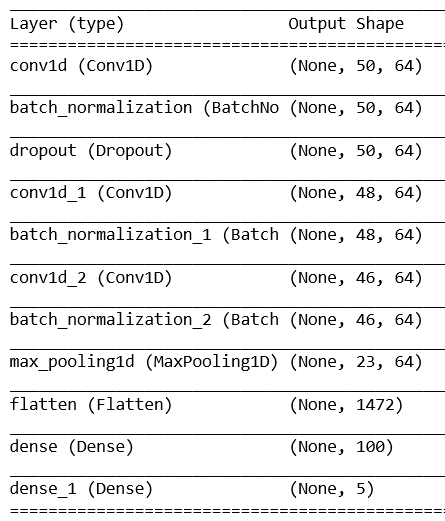
\includegraphics[width=.6\textwidth]{rope_skipping/model_summary.PNG} 
\end{figure}

\subsubsection{Conv1D}
Als eerste wordt gebruik gemaakt van een Conv1D laag. Er werd gekozen voor 1D in plaats van 2D omdat we hier te maken hebben met 1-dimensionale data. Dit is de eerste laag in het model, er moet dus een input\_shape meegegeven worden. De data wordt in segmenten verdeeld met hierin telkens een veelvoud van 52 datapunten, afhankelijk van het gekozen window. 52 Hz is namelijk de gemiddelde frequentie tijdens het datacollectie proces. Elk datapunt bestaat uit 3 dimensies, ook wel \textit{channels} genoemd. De input shape bedraagt bijgevolg (window*52, 3). Er wordt gekozen voor 64 filters. Dit wil zeggen dat de output van deze laag een dimensionality van 64 zal hebben. Als \textit{kernel size} wordt 3 genomen. Dit geeft aan hoe ver de filter zal reiken tijdens het proces van feature extraction en dus in welke mate moet rekening gehouden worden met "context". Ook moet een activatie functie gespecificeerd worden. Ontbreekt deze dan wordt default een lineaire functie gebruikt. Er wordt gekozen voor Relu.
Deze laag wordt meerdere keren toegepast binnen het model, telkens gevolgd door een batchNormalization, aangezien op deze manier meer complexe features kunnen gedetecteerd worden. 

\subsubsection{BatchNormalization}
Vervolgens wordt een BatchNormalization laag ingevoerd. Deze zal ervoor zorgen dat de output van de voorgaande laag genormaliseerd wordt. 
Normalisatie van de trainingsdata is namelijk vereist, maar niet noodzakelijk ten opzichte van ieder afzonderlijk datapunt. Onderstaande Figuren \ref{fig:batchnormalization} en \ref{fig:normalisation} tonen een vergelijking van individuele normalisatie en batchNormalization. Hierbij is het kleine verlies in accuraatheid verwaarloosbaar. Door het invoeren van een batchNormalization laag werd de noodzaak van normalisatie tijdens de preprocessingfase teniet gedaan. Dit is eveneens gunstig voor de implementatie in android.

\begin{figure}[!htpd]
\centering
\begin{floatrow}
  \ffigbox[\FBwidth]{\caption{BatchNormalization}\label{fig:batchnormalization}}{%
    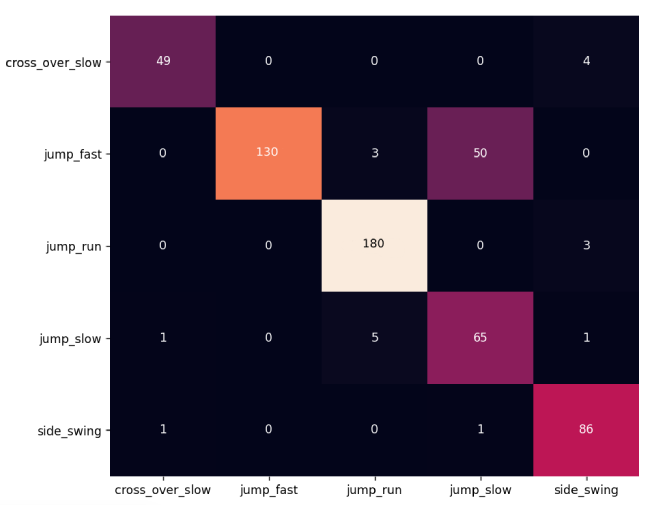
\includegraphics[width=0.5\textwidth]{rope_skipping/batchnormalization.PNG} 
  }
  \ffigbox[\FBwidth]{\caption{Individuele normalisatie}\label{fig:normalisation}}{%
    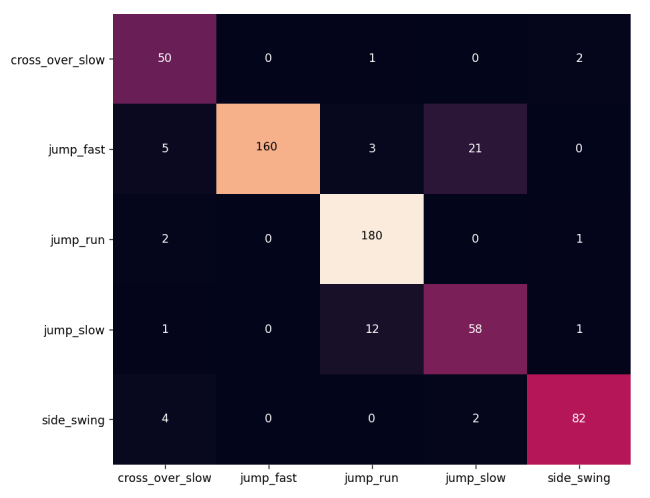
\includegraphics[width=0.5\textwidth]{rope_skipping/normalisatie.PNG}
  }
\end{floatrow}
\end{figure}

\subsubsection{Dropout}
Vervolgens volgt een Dropout laag. Deze laag moet overfitting voorkomen door een bepaald percentage van de input data te negeren. Er wordt gekozen om 30 procent van de datapunten buiten beschouwing te laten.

\subsubsection{MaxPooling1D}
De volgende laag is MaxPooling1D. Deze laag zal ervoor zorgen dat het aantal parameters gereduceerd wordt door telkens enkel de maximum vector te behouden binnen een gebied gedefinieerd door de pool\_size. Hier wordt gekozen voor een pool\_size van 2 en eveneens 2 strides. Dit wil zeggen dat de input gehalveerd zal worden aangezien de filter met grootte 2 telkens met twee eenheden verplaatst wordt.

\subsubsection{Flatten}
De volgende laag is Flatten en doet wat de naam zegt. Het zal de 3D input omvormen naar een 1D vector. Door deze laag toe te passen zal de uiteindelijke output van het model eveneens bestaan uit een 1D array in plaats van een meerdimensionale array.

\subsubsection{Dense/Fully connected}
Als laatste worden twee Dense lagen ingevoerd. De eerste Dense laag zal het dot product uitvoeren tussen de input matrix en de kernel met gewichten. De belangrijkste parameter hier is het aantal neuronen, wat de output shape vastlegt. De tweede dense laag heeft als activatie functie Softmax en zal zorgen voor de classificatie in de verschillende klassen.

\section{Berekeningen}
\subsection{Aantal draaiingen}
Het aantal draaiingen in een rope skipping sessie kan bekomen worden door naar de periode te kijken van het signaal. Deze periode is gelijk over x-, y- en z-as zoals te zien op Figuur \ref{fig:nofilter}. De side swing beweging is hierbij een uitzondering op de regel. De beweging vertoont een verschillend periodiek verloop langs de z-as (zie subsectie \ref{subsection:sideswing}). Eén periode langs deze as omvat een draaibeweging links en rechts van het lichaam. Deze periode wordt aanzien als één draaiing tijdens dit onderzoek. Bijgevolg zal in geval van de side swing beweging enkel rekening gehouden worden met de z-as.
Om het aantal periodes en dus het aantal draaiingen te berekenen, kan één periode manueel uitgesneden worden. Deze wordt dan geconvolueerd met het volledige signaal. De convolutie operatie zal grote pieken vertonen wanneer het signaal overeenkomt. Door deze pieken te tellen, is het aantal periodes en dus het aantal draaiingen geweten. Aangezien de periode voor verschillende sprongen uitgevoerd door verschillende proefpersonen niet telkens een gelijkaardig patroon zal vertonen, is deze manier niet toepasbaar.
Ook kan gekozen worden om de data in het 95\% kwartiel te bekijken. Elke periode heeft namelijk één uitgesproken piek, wat bijgevolg voor een hoge waarde zorgt. De amplitude van het signaal kan echter tijdens een sprong afzwakken of versterken zodat niet elke piek in het 95\% kwartiel voorkomt. Hierdoor is ook dit ook geen optimale methode.
Een laatste poging is om een Savitzky-Golayfilter op het signaal toe te passen. Deze filter zal binnen een vooraf gedefinieerd window een polynomiale functie proberen fitten \cite{ref70}. Een beter resultaat werd bekomen door met verschillende iteraties te werken in plaats van verhoging van het window. Tabel \ref{tab:filter} toont de gebruikte parameters per sprong.

Deze transformatie zal ervoor zorgen dat er per periode slechts één lokaal maxima aanwezig is. Door op dit geëffend signaal een piek detectie uit te voeren kan een vrij goede benadering gemaakt worden van het effectieve aantal draaiingen. Het gemiddelde wordt genomen tussen de drie assen omdat het signaal langs bepaalde assen soms een minder grote amplitude heeft wat kan resulteren in gewijzigde piekdetectie. Ook kan een extra piek, te wijten aan ruis langs een bepaalde as, zorgen voor te veel gedetecteerde draaiingen. Figuur \ref{fig:filter} geeft een gefilterd cross over signaal weer.

\begin{table}[!htpd]
  \centering
  \caption{Savitzky-Golayfilter parameters}
  \label{tab:filter}
\begin{tabular}{lccc}
 \hline \\
\textbf{}             & \textbf{Window} & \textbf{Poly-order } & \textbf{Iteraties} &  \\
\hline \\
\textbf{Jump run}     & 40               & 3            & 2        &  \\
\textbf{Jump slow}    & 50              & 3            & 1        &  \\
\textbf{Jump fast}    & 32               & 5            & 4        &  \\
\textbf{Cross over}   & 40               & 3               & 2        &  \\
\textbf{Side swing}   & 150                  & 5            & 2       & \\\\
\hline \\
\end{tabular}
\end{table}

\begin{figure}[!htpd]
\centering
\caption{Gefilterd signaal}\label{fig:filter}
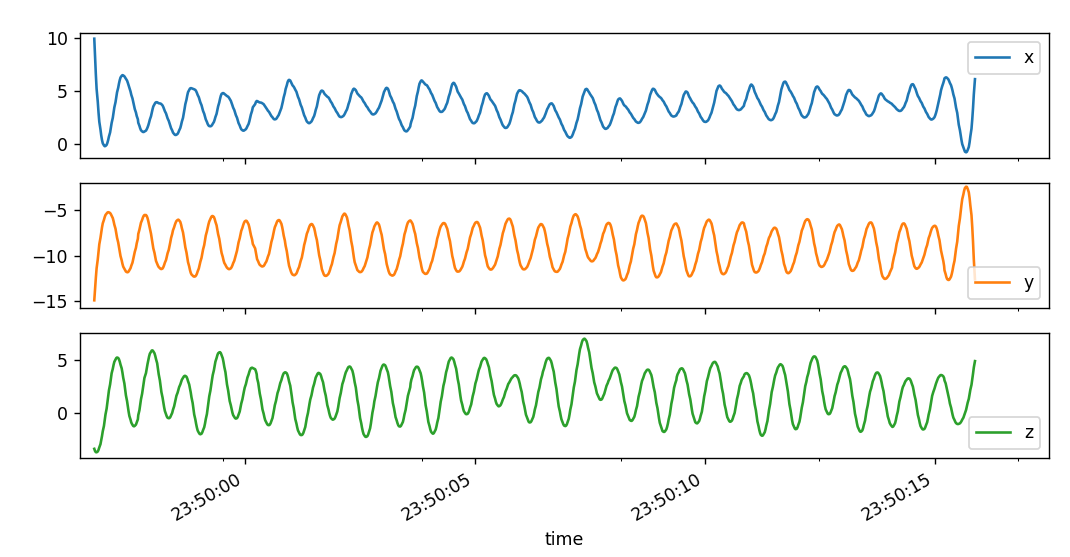
\includegraphics[width=.9\textwidth]{rope_skipping/crossover_gefilt.PNG} 
\end{figure}

\begin{figure}[!htpd]
\centering
\caption{Ongefilterd signaal}\label{fig:nofilter}
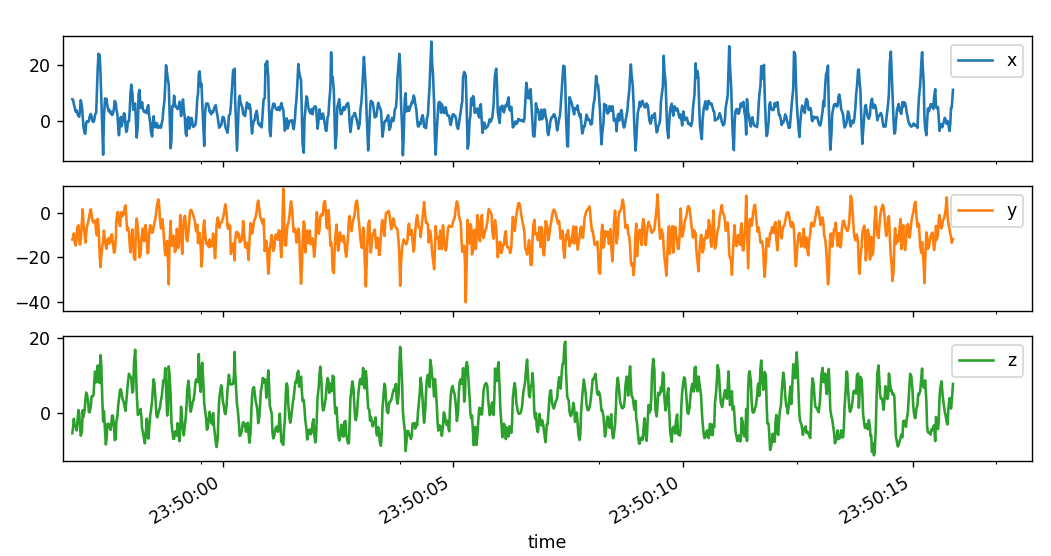
\includegraphics[width=.9\textwidth]{rope_skipping/crossover_nietgefilt.PNG} 
\end{figure}

\subsection{Fouten tijdens een beweging}
Wanneer een fout zich voordoet tijdens een sessie in de vorm van een hapering van het touw, dan is dit duidelijk merkbaar in het verloop van het signaal. Er zal voor enkele seconden geen of amper versnelling zichtbaar zijn. Dit is zichtbaar op Figuur \ref{fig:mistake} Door eerst de afgeleide te nemen van het signaal kan gefilterd worden op datapunten in een interval dichtbij 0. Indien een opeenvolgende reeks genoeg waarden bevat, wordt dit bestempeld als een fout. Via empirisch onderzoek werd deze parameter vastgelegd op 52 datapunten, wat ongeveer een halve seconde betekent. Het foutdetectie interval werd vastgelegd op een ondergrens van 10\% van de laagste en een bovengrens van 10\% van de hoogste piek. Tijdens de evaluatie bleek dat dit bij sprongen met een kleine amplitude een vertekend beeld kan geven vanwege de hogere amplitudes bij het starten met springen. Hierdoor werd gekozen voor een absoluut interval met ondergrens -0.000001 en bovengrens 0.000001.

\begin{figure}[!htpd]
\centering
\caption{Signaal met fout}\label{fig:mistake}
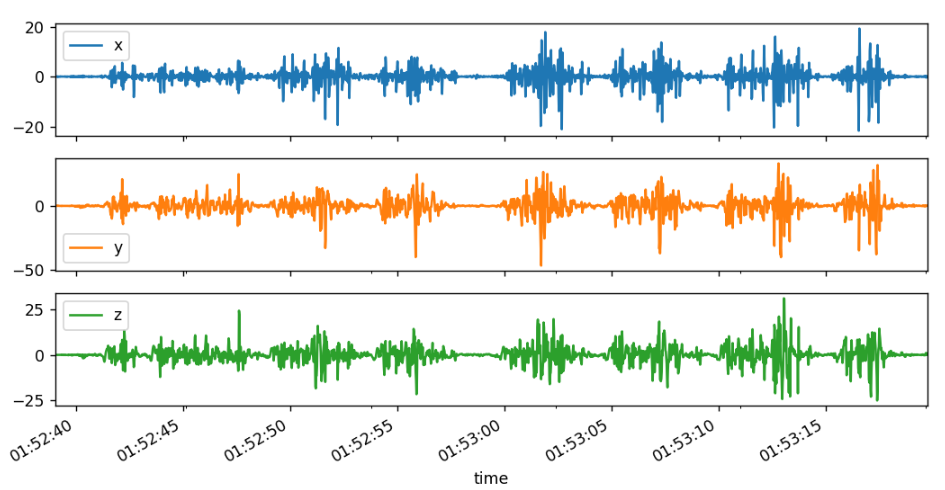
\includegraphics[width=.9\textwidth]{rope_skipping/mistake.PNG} 
\end{figure}